%%%%%%%%%%%%%%%%%%%%%%% file template.tex %%%%%%%%%%%%%%%%%%%%%%%%%
%
% This is a general template file for the LaTeX package SVJour3
% for Springer journals.          Springer Heidelberg 2010/09/16
%
% Copy it to a new file with a new name and use it as the basis
% for your article. Delete % signs as needed.
%
% This template includes a few options for different layouts and
% content for various journals. Please consult a previous issue of
% your journal as needed.
%
%%%%%%%%%%%%%%%%%%%%%%%%%%%%%%%%%%%%%%%%%%%%%%%%%%%%%%%%%%%%%%%%%%%
%
% First comes an example EPS file -- just ignore it and
% proceed on the \documentclass line
% your LaTeX will extract the file if required

%\begin{filecontents*}{example.eps}
%%%!PS-Adobe-3.0 EPSF-3.0
%%%%BoundingBox: 19 19 221 221
%%%%CreationDate: Mon Sep 29 1997
%%%%Creator: programmed by hand (JK)
%%%%EndComments
%gsave
%newpath
%  20 20 moveto
%  20 220 lineto
%  220 220 lineto
%  220 20 lineto
%closepath
%2 setlinewidth
%gsave
%  .4 setgray fill
%grestore
%stroke
%grestore
%\end{filecontents*}

%
\RequirePackage{fix-cm}
%
%\documentclass{svjour3}                     % onecolumn (standard format)
%\documentclass[smallcondensed]{svjour3}     % onecolumn (ditto)
\documentclass[smallextended]{svjour3}       % onecolumn (second format)
%\documentclass[twocolumn]{svjour3}          % twocolumn
%
\smartqed  % flush right qed marks, e.g. at end of proof
%
\usepackage{graphicx}
%
% \usepackage{mathptmx}      % use Times fonts if available on your TeX system
%
% insert here the call for the packages your document requires
%\usepackage{latexsym}
% etc.
%
% please place your own definitions here and don't use \def but
% \newcommand{}{}
%
% Insert the name of "your journal" with
% \journalname{myjournal}
%


\usepackage{bm}
\usepackage{amssymb,amsmath,times,subfigure,tabularx,booktabs,colortbl,multirow,threeparttable}
\usepackage{subfigure}
%\usepackage[notref,notcite]{showkeys}  % use this to temporarily show labels
\usepackage[colorlinks=true, pdfstartview=FitV, linkcolor=black, citecolor= black, urlcolor= black]{hyperref}
%\usepackage{overcite}
%\usepackage{footnpag}			      	% make footnote symbols restart on each page

\usepackage{color}
\usepackage{afterpage}
\newcommand{\hilight}[1]{\colorbox{green}{#1}}

\newtheorem{prop}{Proposition}

\newcommand{\abs}{\mathop{\mathrm{abs}}\nolimits}
\newcommand{\diag}{\mathop{\mathrm{diag}}\nolimits}
\newcommand{\norm}[1]{\ensuremath{\left\| #1 \right\|}}
\newcommand{\bracket}[1]{\ensuremath{\left[ #1 \right]}}
\newcommand{\braces}[1]{\ensuremath{\left\{ #1 \right\}}}
\newcommand{\parenth}[1]{\ensuremath{\left( #1 \right)}}
\newcommand{\pair}[1]{\ensuremath{\langle #1 \rangle}}
\newcommand{\met}[1]{\ensuremath{\langle\langle #1 \rangle\rangle}}
\newcommand{\refeqn}[1]{(\ref{eqn:#1})}
\newcommand{\reffig}[1]{Fig. \ref{fig:#1}}
\newcommand{\tr}[1]{\mathrm{tr}\ensuremath{\negthickspace\bracket{#1}}}
\newcommand{\trs}[1]{\mathrm{tr}\ensuremath{[#1]}}
\newcommand{\ave}[1]{\mathrm{E}\ensuremath{[#1]}}
\newcommand{\deriv}[2]{\ensuremath{\frac{\partial #1}{\partial #2}}}
\newcommand{\dderiv}[2]{\ensuremath{\dfrac{\partial #1}{\partial #2}}}
\newcommand{\SO}{\ensuremath{\mathsf{SO(3)}}}
\newcommand{\T}{\ensuremath{\mathsf{T}}}
\renewcommand{\L}{\ensuremath{\mathsf{L}}}
\newcommand{\so}{\ensuremath{\mathfrak{so}(3)}}
\newcommand{\SE}{\ensuremath{\mathsf{SE(3)}}}
\newcommand{\se}{\ensuremath{\mathfrak{se}(3)}}
\renewcommand{\Re}{\ensuremath{\mathbb{R}}}
\newcommand{\aSE}[2]{\ensuremath{\begin{bmatrix}#1&#2\\0&1\end{bmatrix}}}
\newcommand{\ase}[2]{\ensuremath{\begin{bmatrix}#1&#2\\0&0\end{bmatrix}}}
\newcommand{\D}{\ensuremath{\mathbf{D}}}
\renewcommand{\d}{\ensuremath{\mathfrak{d}}}
\newcommand{\Sph}{\ensuremath{\mathsf{S}}}
\renewcommand{\S}{\Sph}
\newcommand{\J}{\ensuremath{\mathbf{J}}}
\newcommand{\Ad}{\ensuremath{\mathrm{Ad}}}
\newcommand{\intp}{\ensuremath{\mathbf{i}}}
\newcommand{\extd}{\ensuremath{\mathbf{d}}}
\newcommand{\hor}{\ensuremath{\mathrm{hor}}}
\newcommand{\ver}{\ensuremath{\mathrm{ver}}}
\newcommand{\dyn}{\ensuremath{\mathrm{dyn}}}
\newcommand{\geo}{\ensuremath{\mathrm{geo}}}
\newcommand{\Q}{\ensuremath{\mathsf{Q}}}
\newcommand{\G}{\ensuremath{\mathsf{G}}}
\newcommand{\g}{\ensuremath{\mathfrak{g}}}
\newcommand{\Hess}{\ensuremath{\mathrm{Hess}}}

\newcommand{\x}{\ensuremath{\mathbf{x}}}
\renewcommand{\r}{\mathbf{r}}
\renewcommand{\u}{\mathbf{u}}
\newcommand{\y}{\mathbf{y}}

\newcommand{\bfi}{\bfseries\itshape\selectfont}

\graphicspath{{./Figs/}}



\begin{document}

\title{Nonlinear Observability for Relative Orbit Determination with Angles-Only Measurements
\thanks{This research has been supported in part by NSF under the grants CMMI-1243000 (transferred from 1029551), CMMI-1335008, and CNS-1337722.}
}
%\subtitle{Do you have a subtitle?\\ If so, write it here}

%\titlerunning{Short form of title}        % if too long for running head

\author{Evan Kaufman         \and
		T. Alan Lovell         \and
        	Taeyoung Lee
}

%\authorrunning{Short form of author list} % if too long for running head

\institute{E. Kaufman \at
              Dept. of Mechanical and Aerospace Engineering \\
		 The George Washington University \\
		 Washington DC 20052 \\
              Tel.: 216-346-0946\\
              \email{evankaufman@gwu.edu}           %  \\
%             \emph{Present address:} of F. Author  %  if needed
           \and
           T. A. Lovell \at
              Air Force Research Laboratory, Space Vehicles Directorate \\
		 Kirtland AFB, NM\\
		 \email{AFRL.RVSV@kirtland.af.mil}
	    \and
		 T. Lee \at
              Dept. of Mechanical and Aerospace Engineering \\
		 The George Washington University \\
		 Washington DC 20052 \\
              Tel.: 202-994-8710\\
		 Fax: 202-994-0238\\
              \email{tylee@gwu.edu}           %  \\
%             \emph{Present address:} of F. Author  %  if needed
}
\date{Received: date / Accepted: date}
% The correct dates will be entered by the editor


\maketitle

\begin{abstract}
This paper presents nonlinear observability criteria for the relative orbital dynamics represented by the solutions of the two-body problem. It is assumed that a chief is on a circular orbit with a prescribed orbital radius, and it measures lines-of-sight toward a deputy only. A differential geometric method, based on the Lie derivatives, is used to derive sufficient conditions for observability of the orbital properties of the deputy. It is shown that under certain geometric conditions on the relative configuration between the chief and the deputy, the nonlinear relative motion is observable from angles-only measurements. The second part of this paper presents a quantitative measure of observability for the relative orbits, and it is formulated by generalizing the observability Gramian of linear dynamic systems. An extended Kalman filter is also developed to numerically illustrate the observability of nonlinear relative orbits with angles-only measurements and to show correspondence between the proposed observability measure and filtered solution accuracy.


%A new nonlinear observability measure is proposed for relative orbit determination when lines-of-sight between satellites are measured only. It corresponds to a generalization of the observability Gramian in linear dynamic systems to the nonlinear relative orbit dynamics represented by the two-body problems. An extended Kalman filter (EKF) is adapted to this problem and is evaluated with various gravitational harmonics and initial orbital determination (IOD) predictions. Extensive results illustrate correspondence between the proposed observability measure with filtering errors. An extensive numerical analysis in realistic scenarios includes satellite propagation of the two-body problem the $J_2$ perturbation effects.
\keywords{Nonlinear Observability \and Relative Orbit Determination \and Angles-Only Measurements}
% \PACS{PACS code1 \and PACS code2 \and more}
% \subclass{MSC code1 \and MSC code2 \and more}
\end{abstract}

\section{Introduction}

%Space-based surveillance or relative navigation is desirable for many spacecraft missions, such as formation control and rendezvous. Spacecraft maneuvers based only on on-board measurements reduce the total operating cost significantly, and it improves safety against communication interruptions with ground stations. Relative navigation between spacecraft in close-proximity essentially corresponds to space-based orbit determination. In particular, vision-based navigation and estimation of relative orbits have received attention recently, since optical sensors have the desirable properties of low cost and minimal maintenance, while providing accurate line-of-sight measurements, or angles from a chief to a deputy.

Relative orbit determination (ROD) between spacecraft is desirable for many spacecraft missions. In scenarios where the spacecraft are in close-proximity, this is commonly referred to as relative navigation. When baselines between spacecraft are longer, a more appropriate term would be space-based space surveillance or space-based orbit determination. In particular, vision-based ROD has received attention recently, since optical sensors have the desirable properties of being low cost and minimal maintenance, while providing accurate line-of-sight measurements, or angles, from a chief to a deputy.

ROD based on angles-only measurements has been investigated in \cite{WofGelITAES09,PatLovPASFMM12}. The problem is to determine the relative orbit between a chief spacecraft and a deputy spacecraft by using the line-of-sight between the two objects, assuming that the orbit of the chief is prescribed exactly. Reference \cite{WofGelITAES09} shows that the relative orbit is unobservable from angles-only measurements when linear relative orbital dynamics are assumed, unless there are thrusting maneuvers. Reference~\cite{PatLovPASFMM12} introduces the concept of partial observability to determine a basis vector representing a family of relative orbits, and an initial orbit determination technique is developed for this method. Linear observability analysis is performed numerically for a particular case in~\cite{YimCraPASMM04}. 

All of the above results are based on linear relative orbital dynamics.
%It is straightforward to see that the relative orbit is not observable with angles-only measurements through its linearized dynamics. In other words,
Under these assumptions, there are an infinite number of relative orbits that yield identical line-of-sight measurements, and therefore the orbital distance between a deputy and a chief cannot be determined by angles-only measurements. As such, it is required to study the nonlinear relative orbital dynamics to determine observability with angles-only measurements. 

%Recently, observability criteria have been derived for the nonlinear relative orbital dynamics represented by the solutions of the two-body problem without linearization~\cite{LovLeePISSFD14}.

This paper constructs observability criteria for the nonlinear relative orbital dynamics represented by the two-body problem without linearization. Assuming that a chief is on a circular orbit with a prescribed orbital radius, nonlinear equations of motion for the relative orbital motion of a deputy with respect to the chief are presented. A differential geometric method, based on the Lie derivatives of the line-of-sight from the chief to the deputy~\cite{HerKreITAC77}, is applied to obtain sufficient conditions for observability, under the assumptions of these equations. It is shown that under certain geometric conditions on the relative configuration between the chief and the deputy, the relative motion is observable from angles-only measurements if nonlinear dynamics are assumed.

Next, we present a new measure of observability for relative orbit determination with angles-only measurements. This is motivated to understand the degree of observability for the relative orbital dynamics, and to identify the class of relative orbits that have stronger or weaker observability. For a given initial condition of relative orbits, the proposed observability measure determines how much the corresponding relative orbits are easy or difficult to estimate, thereby providing a quantitative measure for relative orbit determination.

The last part of this paper is focused on a feasibility study of an extended Kalman filter (EKF) for orbit determination using angles-only measurements in realistic scenarios. The filtering performances of the EKF are studied for several types of relative orbits to show nonlinear observability with angles-only measurements explicitly, and they are compared with the proposed observability measure. Additional cases with $J_2$ perturbations are also considered to identify the effects of orbital perturbations. 

In short, the main contributions of this paper are constructing sufficient conditions for the observability of nonlinear relative orbits with angles-only measurements that have not been studied before, and proposing a new quantitative measure of observability. 

This paper is organized as follows. The relative orbital dynamics and the orbit determination problem are formulated in Section 2. Observability criteria and an observability measure are presented in Section 3 and Section 4, respectively, which are followed by numerical examples and conclusions.

%The filter is subject to measurement uncertainty and perturbation forces not considered with the two-body problem, on which the filter is based. Then, the performance of the EKF is compared with the proposed observability measure to show the correspondence. 

\section{Nonlinear Relative Orbital Dynamics}\label{sec:ND}

Consider two satellites orbiting around the Earth, referred to as a \textit{chief} and a \textit{deputy}. Suppose that the chief satellite is on a circular orbit with a pre-determined orbital radius of $a\in\Re$.

Define a local-vertical, local-horizontal (LVLH) frame as follows. Its origin is located at the chief satellite. The $x$-axis is along the radial direction from the Earth to the chief, and the $y$-axis is along the velocity vector of the chief. The $z$-axis is normal to the orbital plane, and it is parallel to the angular momentum vector of the chief. The LVLH frame is rotating with the angular velocity of $\mathbf{\omega}=[0,0,n]^T\in\Re^3$, where $n=\sqrt{\frac{\mu}{a^3}}$ is the mean motion of the chief satellite, and $\mu$ denotes the gravitational parameter of the Earth. Note that the inertial velocity of the chief expressed in LVLH coordinates is given by $\mathbf{v}_{chief}=[0,na,0]^T\in\Re^3$. Let the relative position of the deputy satellite with respect to the chief be given by $\mathbf{r}=[x,y,z]^T\in\Re^3$ in the LVLH frame. 

\subsection{Nonlinear Equations of Motion}

Nonlinear equations of motion for the relative motion of the deputy with respect to the chief can be derived as follows based on Lagrangian mechanics~\cite{LovLeePISSFD14}. 

Considering that the LVLH frame is rotating with the angular velocity of $\mathbf{\omega}=[0,0,n]^T$, the inertial velocity of the deputy satellite expressed in LVLH coordinates is given by
\begin{align*}
\mathbf{v}_{deputy}
=
\mathbf{v}_{chief} + \dot{\r} + \mathbf{\omega}\times \mathbf{r} = 
\begin{bmatrix}
0 \\ na \\ 0
\end{bmatrix}
+
\begin{bmatrix}
\dot x \\ \dot y \\ \dot z
\end{bmatrix}
+
\begin{bmatrix}
-n y \\ nx \\ 0
\end{bmatrix}
=
\begin{bmatrix}
\dot x - ny \\ \dot y + nx + na \\ \dot z
\end{bmatrix}.
\end{align*}
Therefore, the (normalized) kinetic energy of the deputy satellite is 
\begin{align*}
T = \frac{1}{2}\|\mathbf{v}_{deputy}\|^2 = \frac{1}{2} \braces{(\dot x -ny)^2+(\dot y + nx +na)^2 + \dot z^2}.
\end{align*}
The location of the Earth from the chief is given by $[-a,0,0]^T$ in the LVLH frame. Therefore, the position vector of the deputy from the center of the Earth is given by 
$\r_a=[x+a,y,z]^T\in\Re^3$. The gravitational potential energy is 
\begin{align*}
U = -\frac{\mu}{\sqrt{(x+a)^2 + y^2 + z^2}} = -\frac{\mu}{\|\r_a\|}.
\end{align*}
From the above equations, the Lagrangian of the deputy satellite is expressed as $L(x,y,z,\dot x,\dot y ,\dot z) = T(x,y,\dot x,\dot y,\dot z)- U(x,y,z)$. Using the Euler-Lagrange equations, given by
\begin{align*}
\frac{d}{dt}\deriv{L}{\dot q}-\deriv{L}{q}=0,
\end{align*}
for $q\in\{x,y,z\}$, we obtain the nonlinear equations of motion for the relative orbit as follows.
\begin{align}
\ddot x - 2n\dot y -n^2 x&=n^2 a - \frac{\mu (x+a)}{((x+a)^2 + y^2 + z^2)^{3/2}},\label{eqn:ddotx}\\
\ddot y + 2n\dot x -n^2 y &=   - \frac{\mu y}{((x+a)^2 + y^2 + z^2)^{3/2}},\label{eqn:ddoty}\\
\ddot z &= - \frac{\mu z}{((x+a)^2 + y^2 + z^2)^{3/2}}.\label{eqn:ddotz}
\end{align}

These can be written as the standard form of the nonlinear state equation,
\begin{align}
\dot{\mathbf{x}} = f (\mathbf{x}), \label{eqn:xxdot}
\end{align}
where the state vector is $\mathbf{x}=[x,y,z,\dot x, \dot y,\dot z]^T\in\Re^N$ with $N=6$, and
\begin{align}
f(\mathbf{x}) 
%= \begin{bmatrix}
%\dot x\\
%\dot y\\
%\dot z\\
%2n\dot y +n^2 (x+a) - \dfrac{\mu (x+a)}{((x+a)^2 + y^2 + z^2)^{3/2}}\\
%-2n\dot x +n^2 y  - \dfrac{\mu y}{((x+a)^2 + y^2 + z^2)^{3/2}}\\
%- \dfrac{\mu z}{((x+a)^2 + y^2 + z^2)^{3/2}}
%\end{bmatrix}
=\begin{bmatrix}
\dot \r \\
-2\omega\times \dot\r - \omega\times(\omega\times \r_a) -\dfrac{\mu \r_a}{\|\r_a\|^3}
\end{bmatrix}.\label{eqn:f}
\end{align}
%where $\r=[x,y,z]^T\in\Re^3$, $\r_a = [x+a,y,z]^T\in\Re^3$, and $\dot\r =[\dot x,\dot y,\dot x]^T\in\Re^3$. 

\subsection{Line-of-sight Measurement}

We assume that the line-of-sight from the chief to the deputy is measured by onboard sensors, such as optical sensors. The measurement is represented by the unit-vector along the relative position vector, i.e.,
\begin{align}
\y = h(\mathbf{x}) =\frac{\r}{\|\r\|},\label{eqn:y}
\end{align}
where $\y\in\Re^3$, and it satisfies $\|\y\|=1$.

\section{Nonlinear Observability Criteria}\label{sec:OC}

Based on the nonlinear dynamic model presented in the previous section, here we derive sufficient conditions for the observability of the relative orbit with line-of-sight measurements.



\subsection{Observability Criteria for Nonlinear Systems}



Observability of nonlinear systems and sufficient conditions for observability are summarized as follows~\cite{HerKreITAC77,Nijvan90}. For a given nonlinear dynamic system described with \refeqn{xxdot} and \refeqn{y}, a pair of points $\x_0$ and $\x_1$ is called \textit{indistinguishable} if the outputs of the corresponding solutions starting from each of $\x_0$ and $\x_1$ are identical for a certain time period. Note that $\x_0$ is indistinguishable from $\x_0$ trivially from the definition. The system is \textit{locally weakly observable} at $\x_0$, if there exists an open neighborhood $V$ of $\x_0$ such that for every open neighborhood $V_0$ of $\x_0$ contained in $V$, the only indistinguishable point to $\x_0$ is the point $\x_0$ itself. This implies that $\x_0$ is distinguishable from any other points in a neighborhood of it.

Next, sufficient conditions for observability are presented. The Lie-derivative of the output $h(\x)$ along $f(\x)$, namely $L_f h(\x)$ is defined as follows:
\begin{align*}
L_f h(\x) = \deriv{h(\x)}{\x}f(\x)\in\Re^{M\times 1},
\end{align*}
which corresponds to the directional derivative of $h(\x)$ along $f(\x)$, and $\deriv{h(\x)}{\x}\in\Re^{M\times N}$. For a non-negative integer $i$, the $i$-th order Lie-derivative is defined by induction as $L_f^i h = L_f (L_f^{i-1} h)$ with $L_f^0 h = h$. For a positive integer $k$, define a $k$-th order observability matrix $\mathcal{O}\in\Re^{kM\times N}$ as
\begin{align*}
\mathcal{O}(\x_0) = \deriv{}{\x} \begin{bmatrix} L_f^0 h(\x) \\ L_f^1 h(\x)\\ \vdots \\L_f^{k} h(\x)\end{bmatrix}\Bigg|_{\x=\x_0}.
\end{align*}
It has been shown that the system is locally weakly observable at $\x_0$ if the rank of the observability matrix $\mathcal{O}(\x_0) = N$ for some $k$~\cite{HerKreITAC77,Nijvan90}. When applied to linear dynamics, this yields the well-known observability rank condition for linear systems. 

In general, the order $k$ of the observability should be increased until the rank condition is satisfied. Note that when there is more than a single measurement type for each measurement time, i.e., $M>1$, it is possible to satisfy the observability rank condition without need for computing the higher-order Lie derivatives up to the $N-1$-th order.

\subsection{Observability Criteria for Relative Orbital Dynamics}

\paragraph{Observability Matrix}
We apply the above observability criteria for the nonlinear relative orbital dynamics. The first block of rows of the observability matrix is simply given by
\begin{align*}
\deriv{}{\x} L_f^0 h(\x) = \deriv{\y}{\x}.
\end{align*} 
Similarly, from \refeqn{xxdot}, the second row block is
\begin{align*}
\deriv{}{\x} L_f^1 h(\x) = \deriv{}{\x}\parenth{\deriv{\y}{\x}f(\x)}=\deriv{\dot\y}{\x}.
\end{align*} 
Since $\dot\y$ is determined completely from $\x$, we have
\begin{align*}
\deriv{}{\x} L_f^2 h(\x) = \deriv{}{\x}\parenth{\deriv{\dot\y}{\x}f(\x)}=\deriv{\ddot\y}{\x}.
\end{align*}
Using these and the fact that $\x=[\r^T,\dot \r^T]$, the observability matrix of the relative orbital dynamics can be written as
\begin{align}
\mathcal{O} =
\begin{bmatrix}
\deriv{\y}{\r} & \deriv{\y}{\dot\r}\\
\deriv{\dot\y}{\r} & \deriv{\dot\y}{\dot\r}\\
\deriv{\ddot\y}{\r} & \deriv{\ddot\y}{\dot\r}
\end{bmatrix}
\triangleq
\begin{bmatrix}
\mathcal{O}_{00} & 0_{3\times 3}\\
\mathcal{O}_{10} & \mathcal{O}_{11}\\
\mathcal{O}_{20} & \mathcal{O}_{21}
\end{bmatrix}\in\Re^{9\times 6},\label{eqn:OO}
\end{align}
where the submatrices $\mathcal{O}_{ij}\in\Re^{3\times 3}$ are defined for each block, and we used the fact that the measurement $\y$ is independent of $\dot\r$. Here we consider the observability matrix obtained by up to the second order Lie derivatives of the measurement due to complexity. But, this still provides sufficient conditions for observability under certain geometric conditions described later. %asdf

After straightforward but tedious algebraic manipulations using the following identity repeatedly,
\begin{align*}
\delta \parenth{\frac{1}{\|\mathbf{r}\|^i}} 
& = -i\frac{ \mathbf{r}^T \delta \mathbf{r}}{\|\mathbf{r}\|^{i+2}},
\end{align*}
for any positive integer $i$, we can show that the submatrices $\mathcal{O}_{ij}$ of the observability matrix $\mathcal{O}$ are given by
\begin{align}
\mathcal{O}_{00} & = \deriv{\y}{\r} = \frac{1}{\|\r\|}(I - \y\y^T),\label{eqn:O_00}\\
\mathcal{O}_{10} & = \deriv{\dot\y}{\r} = \deriv{}{\r} \parenth{\deriv{\y}{\r}\dot \r}= -\frac{1}{\|\r\|^2}\braces{
{\dot\r\y^T +\y^T\dot\r I +\y\dot\r^T}
- 3\y\y^T\dot\r \y^T},\\
\mathcal{O}_{11} & = \deriv{\dot\y}{\dot\r} = \deriv{}{\dot\r} \parenth{\deriv{\y}{\r}\dot \r}= \deriv{\y}{\r} = \mathcal{O}_{00},\label{eqn:O11}\\
\mathcal{O}_{20} & = \deriv{\ddot\y}{\r} = -\dfrac{2\dot\r \dot\r^T  +\dot\r^T\dot\r I}{\|\r\|^3}
+3\dfrac{2(\r^T\dot\r) \dot\r\r^T +(\dot\r^T\dot\r)\r\r^T
+(\r^T\dot\r)^2 I
+2(\r^T\dot\r)\r  \dot\r^T
}{\|\r\|^5}\nonumber \\
&\quad- 15 \dfrac{(\r^T\dot\r)^2\r  \r^T}{\|\r\|^7}
-\dfrac{\ddot{\r}\r^T +\r^T\ddot{\r} I +\r \ddot{\r}^T}{\|\r\|^3}
+ 3 \dfrac{(\r^T\ddot{\r})\r \r^T}{\|\r\|^5}\nonumber\\
&\quad+\parenth{\dfrac{I}{\|\mathbf{r}\|} - \dfrac{\mathbf{r}\mathbf{r}^T}{\|\mathbf{r}\|^3}}
\parenth{-[\omega]_\times^2 -\dfrac{\mu I_{3\times 3}}{\|\r_a\|^3} + \dfrac{3\mu\r_a\r_a^T}{\|\r_a\|^5}},\\
\mathcal{O}_{21} & = \deriv{\ddot\y}{\dot\r} = \deriv{}{\dot\r}\parenth{\deriv{}{\r}\parenth{\deriv{\y}{\r}\dot\r}\dot\r + \deriv{\y}{\r}\ddot\r} = 2 \deriv{}{\r} \parenth{\deriv{\y}{\r}\dot\r} + \deriv{\y}{\r} \deriv{\ddot\r}{\dot\r}
\nonumber\\
&  = 2\mathcal{O}_{10} 
- 2 \mathcal{O}_{00}[\omega]_\times,\label{eqn:O_21}
\end{align}
where $[\omega]_\times\in\Re^{3\times 3}$ is defined as
\begin{align*}
[\omega]_\times = \begin{bmatrix} 0 & -n & 0 \\ n & 0 & 0 \\ 0 & 0 & 0 \end{bmatrix}.
\end{align*}
These expressions have been verified by the Matlab symbolic computation toolbox.

After some algebraic manipulations, we can show that the submatrices satisfy the following identities, 
\begin{align}
\mathcal{O}_{10}\r & = 
%-\frac{1}{\|\r\|}\braces{{\dot\r\y^T +\y^T\dot\r I +\y\dot\r^T}- 3\y\y^T\dot\r \y^T}\y\\
%&=-\frac{1}{\|\r\|}\braces{\dot\r +(\y^T\dot\r)\y +\y(\dot\r^T\y)- 3\y(\y^T\dot\r) }\\
%&=-\frac{1}{\|\r\|}\braces{\dot\r -\y(\y^T\dot\r) }=
-\mathcal{O}_{00}\dot\r,\label{eqn:O10r}\\
\mathcal{O}_{10}\dot\r & = -\frac{1}{\|\r\|^2}\braces{
{2\dot\r(\y^T\dot \r)  +\y(\dot\r^T\dot \r)}
- 3\y(\y^T\dot\r)^2},\label{eqn:O10dotr}\\
\mathcal{O}_{20}\r %& = 
%-\dfrac{2\dot\r \dot\r^T\y  +\dot\r^T\dot\r \y}{\|\r\|^2}
%+3\dfrac{2(\y^T\dot\r) \dot\r\y^T\y +(\dot\r^T\dot\r)\y\y^T\y+(\y^T\dot\r)^2 y +2(\y^T\dot\r)\y \dot\r^T\y}{\|\r\|^2}
%- 15 \dfrac{(\y^T\dot\r)^2\y  \y^T\y}{\|\r\|^2}\nonumber \\
%&\quad -\dfrac{\ddot{\r}\y^Ty +\y^T\ddot{\r} \y +\y \ddot{\r}^T\y}{\|\r\|^1}
%+ 3 \dfrac{(\y^T\ddot{\r})\y \y^T\y}{\|\r\|}
%+\parenth{\dfrac{I}{\|\mathbf{r}\|} - \dfrac{\mathbf{r}\mathbf{r}^T}{\|\mathbf{r}\|^3}}
%\parenth{-[\omega]_\times^2 -\dfrac{\mu I_{3\times 3}}{\|\r_a\|^3} + \dfrac{3\mu\r_a\r_a^T}{\|\r_a\|^5}}\r,\\
%&=
%-\dfrac{2\dot\r (\dot\r^T\y)  +(\dot\r^T\dot\r) \y}{\|\r\|^2}
%+3\dfrac{2(\y^T\dot\r) \dot\r +(\dot\r^T\dot\r)\y+(\y^T\dot\r)^2 \y +2(\y^T\dot\r)^2\y }{\|\r\|^2}
%- 15 \dfrac{(\y^T\dot\r)^2\y}{\|\r\|^2}\nonumber \\
%&\quad -\dfrac{\ddot{\r} +(\y^T\ddot{\r}) \y +\y (\ddot{\r}^T\y)}{\|\r\|^1}
%+ 3 \dfrac{(\y^T\ddot{\r})\y }{\|\r\|}
%+\parenth{\dfrac{I}{\|\mathbf{r}\|} - \dfrac{\mathbf{r}\mathbf{r}^T}{\|\mathbf{r}\|^3}}
%\parenth{-[\omega]_\times^2 -\dfrac{\mu I_{3\times 3}}{\|\r_a\|^3} + \dfrac{3\mu\r_a\r_a^T}{\|\r_a\|^5}}\r,\\
%&=
%-\dfrac{2\dot\r (\dot\r^T\y)  +(\dot\r^T\dot\r) \y}{\|\r\|^2}
%+3\dfrac{2(\y^T\dot\r) \dot\r +(\dot\r^T\dot\r)\y+(\y^T\dot\r)^2 \y +2(\y^T\dot\r)^2\y }{\|\r\|^2}
%- 15 \dfrac{(\y^T\dot\r)^2\y}{\|\r\|^2}\nonumber \\
%&\quad -\dfrac{\ddot{\r} +(\y^T\ddot{\r}) \y +\y (\ddot{\r}^T\y)}{\|\r\|^1}
%+ 3 \dfrac{(\y^T\ddot{\r})\y }{\|\r\|}
%+\parenth{\dfrac{I}{\|\mathbf{r}\|} - \dfrac{\mathbf{r}\mathbf{r}^T}{\|\mathbf{r}\|^3}}
%\parenth{-[\omega]_\times^2 -\dfrac{\mu I_{3\times 3}}{\|\r_a\|^3} + \dfrac{3\mu\r_a\r_a^T}{\|\r_a\|^5}}\r,\\
%&=
%\dfrac{4\dot\r (\dot\r^T\y)  -2(\dot\r^T\dot\r)\y-6(\y^T\dot\r)^2 \y }{\|\r\|^2}
% -\mathcal{O}_{00}\ddot \r
%+\parenth{\dfrac{I}{\|\mathbf{r}\|} - \dfrac{\mathbf{r}\mathbf{r}^T}{\|\mathbf{r}\|^3}}
%\parenth{-[\omega]_\times^2 -\dfrac{\mu I_{3\times 3}}{\|\r_a\|^3} + \dfrac{3\mu\r_a\r_a^T}{\|\r_a\|^5}}\r,\\
& = -2\mathcal{O}_{10}\dot\r +\mathcal{O}_{00}\braces{-\ddot \r +\deriv{\ddot\r}{\r}\r},\label{eqn:O20r}\\
\mathcal{O}_{21}\r & = -2\mathcal{O}_{00} (\dot\r+\omega\times\r),\label{eqn:O21r}\\
\mathcal{O}_{21}\dot\r & = 2\mathcal{O}_{10} \dot\r
- 2 \mathcal{O}_{00}[\omega]_\times\dot\r,\label{eqn:O21rdot}
\end{align}
which are useful to derive the observability criteria. 

\paragraph{Observability Rank Condition}



Now we present sufficient conditions that the observability matrix $\mathcal{O}$ has the full rank of six. 

\begin{prop}
Define three vectors $\mathbf{v}_{rel}$, $\mathbf{a}_1,\mathbf{a}_2\in\Re^3$ as 
\begin{align}
\mathbf{v}_{rel} & = \dot\r +\omega\times\r,\label{eqn:vrel}\\
\mathbf{a}_1 & = \ddot\r-\deriv{\ddot\r}{\r}\r = -2\omega\times \dot\r - [\omega]_\times^2 a \mathbf{e}_1 -\dfrac{\mu a }{\|\r_a\|^3}\mathbf{e}_1- \dfrac{3\mu\r_a^T\r}{\|\r_a\|^5}\r_a,\label{eqn:a1}\\
\mathbf{a}_2 & = \ddot\r-\deriv{\ddot\r}{\r}\r -\deriv{\ddot\r}{\dot\r}\dot\r = \mathbf{a}_1+2\omega\times\dot\r= - [\omega]_\times^2 a \mathbf{e}_1 -\dfrac{\mu a }{\|\r_a\|^3}\mathbf{e}_1- \dfrac{3\mu\r_a^T\r}{\|\r_a\|^5}\r_a,\label{eqn:a2}
\end{align}
where $\mathbf{e}_1=[1,0,0]^T\in\Re^3$ and $\r_a=[x+a,y,z]^T\in\Re^3$. The nonlinear relative orbital dynamics are locally weakly observable at $\x=[\r^T,\dot\r^T]$ if
%\begin{list}{}{\setlength{\leftmargin}{1cm}\setlength{\itemsep}{0mm}\setlength{\parsep}{0mm}\setlength{\topsep}{0mm}\setlength{\parskip}{0mm}\setlength{\labelwidth}{2cm}}
%\item[(i)] when $\r\times\dot\r =0$, $\r\times\mathbf{a}_1\neq 0$ and $\r^T(\mathbf{v}_{rel}\times \mathbf{a}_1)\neq 0$,
%\item[(ii)] when $\r\times\dot\r \neq 0$, $\r\times\mathbf{a}_2\neq 0$ and $\r^T(\mathbf{v}_{rel}\times \mathbf{a}_2)\neq 0$.
%\end{list}
%\begin{alignat}{2}
%(i)&\; &\text{when $\r\times\dot\r =0$, $\r\times\mathbf{v}_{rel}\neq0$, $\r\times\mathbf{a}_1\neq 0$,  and $\r^T(\mathbf{v}_{rel}\times \mathbf{a}_1)\neq 0$},\label{eqn:cond1}\\
%(ii)& &\text{when $\r\times\dot\r \neq 0$, $\r\times\mathbf{v}_{rel}\neq0$, $\r\times\mathbf{a}_2\neq 0$ and $\r^T(\mathbf{v}_{rel}\times \mathbf{a}_2)\neq 0$.}\label{eqn:cond2}
%\end{alignat}
\begin{itemize}
\item[(i)] when $\r\times\dot\r =0$, 
\begin{gather}
\r\times\mathbf{v}_{rel}\neq0,\; \r\times\mathbf{a}_1\neq 0,\; \text{ and } \r^T(\mathbf{v}_{rel}\times \mathbf{a}_1)\neq 0,\label{eqn:cond1}
\end{gather}
\item[(ii)] when $\r\times\dot\r \neq 0$, 
\begin{gather}
\r\times\mathbf{v}_{rel}\neq0,\; \r\times\mathbf{a}_2\neq 0,\; \text{ and } \r^T(\mathbf{v}_{rel}\times \mathbf{a}_2)\neq 0.\label{eqn:cond2}
\end{gather}
\end{itemize}

\end{prop}

\begin{proof}
We show that if the above conditions are satisfied, then the six columns of the observability matrix are linearly independent. Suppose that for a constant vector $\mathbf{c}=[\mathbf{c}_1^T,\mathbf{c}_2^T]\in\Re^6$, where $\mathbf{c}_1,\mathbf{c}_2\in\Re^3$, we have $\mathcal{O}\mathbf{c}=0$, i.e., 
\begin{align}
\mathcal{O} \mathbf{c} = \begin{bmatrix}
\mathcal{O}_{00} & 0_{3\times 3}\\
\mathcal{O}_{10} & \mathcal{O}_{11}\\
\mathcal{O}_{20} & \mathcal{O}_{21}
\end{bmatrix}
\begin{bmatrix} \mathbf{c}_1 \\ \mathbf{c}_2 \end{bmatrix}
=
\begin{bmatrix}
\mathcal{O}_{00}\mathbf{c}_1\\
\mathcal{O}_{10}\mathbf{c}_1+ \mathcal{O}_{11}\mathbf{c}_2\\
\mathcal{O}_{20}\mathbf{c}_1+ \mathcal{O}_{21}\mathbf{c}_2
\end{bmatrix}
=
\begin{bmatrix}
0_{3\times 1}\\
0_{3\times 1}\\
0_{3\times 1}
\end{bmatrix}.\label{eqn:Oc}
\end{align}

We wish to show that there is no non-zero vector $\mathbf{c}$ satisfying \refeqn{Oc} under the given conditions. In the first three rows of \refeqn{Oc}, we have
\begin{align}
\mathcal{O}_{00} \mathbf{c}_1 = \frac{1}{\|\r\|}(I-\y\y^T) \mathbf{c}_1 = 0.\label{eqn:c10}
\end{align}
The matrix $\mathcal{O}_{00}$ has a one-dimensional null space spanned by $\y$. Therefore, without loss of generality, we can choose $\mathbf{c}_1=0$ or $\mathbf{c}_1=\r$. As we are interested in any non-zero vector satisfying the above equation, let $\mathbf{c}_1=\r$ for the subsequent development.

For the chosen value of $\mathbf{c}_1=\r$, we find the next three rows of \refeqn{Oc} as
\begin{align}
\mathcal{O}_{10} \mathbf{c}_1 +\mathcal{O}_{11} \mathbf{c}_2 & = \mathcal{O}_{10} \r +\mathcal{O}_{11} \mathbf{c}_2  = \mathcal{O}_{00} (-\dot\r + \mathbf{c}_2)\nonumber\\
& = \frac{1}{\|\r\|}(I-\y\y^T)(-\dot\r + \mathbf{c}_2)=0,\label{eqn:row2}
\end{align}
where we have used \refeqn{O11} and \refeqn{O10r}. Next, we consider two cases of \refeqn{row2}, namely (i) when $\r\times\dot\r=0$, and (ii) when $\r\times\dot\r\neq 0$. For each case, we show that $\mathbf{c}=0$ to satisfy \refeqn{Oc} under the given sufficient conditions.

\paragraph{Case (i): $\r\times\dot \r=0$} In this case, $\dot \r$ can be written as $\dot \r = \alpha\r$ for some constant $\alpha$ as $\r$ is parallel to $\dot\r$. Then, \refeqn{row2} reduces to 
\begin{align*}
\frac{1}{\|\r\|}(I-\y\y^T)\mathbf{c}_2=0,
\end{align*}
which implies that $\mathbf{c}_2= c\r$ for an arbitrary constant $c$. For the given choice of $\mathbf{c}=[\r^T,c\r^T]^T$, the last three rows of \refeqn{Oc} are given by
\begin{align*}
\mathcal{O}_{20} \mathbf{c}_1 +\mathcal{O}_{21} \mathbf{c}_2 
& = \mathcal{O}_{20} \r + c\mathcal{O}_{21} \r.
\end{align*}
Using \refeqn{O20r} and \refeqn{O21r}, this can be rewritten as
\begin{align*}
\mathcal{O}_{20} \mathbf{c}_1 +\mathcal{O}_{21} \mathbf{c}_2 
& =
-2\mathcal{O}_{10}\dot\r +\mathcal{O}_{00}\braces{-\ddot \r +\deriv{\ddot\r}{\r}\r}
-2c\mathcal{O}_{00} (\dot\r+\omega\times\r).
\end{align*}
But, from \refeqn{O10dotr}, we can show that $2\mathcal{O}_{10}\dot\r=0$ when $\r$ is parallel to $\dot \r$. Using \refeqn{vrel} and \refeqn{a1}, this further reduces to
\begin{align}
\mathcal{O}_{20} \mathbf{c}_1 +\mathcal{O}_{21} \mathbf{c}_2 
& =
-\mathcal{O}_{00}(\mathbf{a}_1 +2c \mathbf{v}_{rel})\nonumber\\
& = - \frac{1}{\|\r\|}(I-\y\y^T)(\mathbf{a}_1 +2c \mathbf{v}_{rel})=0.\label{eqn:row3i}
\end{align}
The matrix $(I-\y\y^T)$ represents the orthogonal projection of a vector into the plane normal to $\y$. From the second condition of \refeqn{cond1}, namely $\r\times\mathbf{a}_1\neq 0$, we have $(I-\y\y^T)\mathbf{a}_1\neq 0$, which implies that the constant $c$ cannot be simply chosen as $c=0$. Therefore, the only possible case to satisfy the above equation is when $\mathbf{a}_1 +2c \mathbf{v}_{rel}$ is parallel to $\r$ for some values of $c$. However, that is not feasible since the third condition of \refeqn{cond1}, namely $\r^T(\mathbf{v}_{rel}\times\mathbf{a}_1)\neq0$, implies that the three vectors $\r$, $\mathbf{a}_1$, and $\mathbf{v}_{rel}$ do not belong to a common plane, i.e., there is no constant $c$ such that $\mathbf{a}_1 +2c \mathbf{v}_{rel}$ is parallel to $\r$.

Therefore, there is no $\mathbf{c}\in\Re^6$ satisfying \refeqn{Oc} if $\mathbf{c}_1=\r$, under the given condition \refeqn{cond1}. This implies that $\mathbf{c}_1=0$ from \refeqn{c10}. Substituting this back into \refeqn{Oc}, we have $\mathcal{O}_{11}\mathbf{c}_2=\mathcal{O}_{00}\mathbf{c}_2=0$, which follows that $\mathbf{c}_2=c\r$ for some constant $c$. However, when $\mathbf{c}_2=c\r$, the last three rows of \refeqn{Oc} are given by
\begin{align}
\mathcal{O}_{21}\mathbf{c}_2 = 2c(\mathcal{O}_{10}-\mathcal{O}_{00}[\omega]_\times) \r
= -2c\mathcal{O}_{00}\mathbf{v}_{rel}=0,\label{eqn:row3i1}
\end{align}
where \refeqn{O10r} is used. But, from the first condition of \refeqn{cond1}, we have $\mathcal{O}_{00}\mathbf{v}_{rel}\neq 0$, and therefore $c=0$, i.e., $\mathbf{c}_2=c\r =0$.

In short, under the given condition \refeqn{cond1}, the equation \refeqn{Oc} implies that $\mathbf{c}=0$. Therefore, the six columns of the observability matrix $\mathcal{O}$ are linearly independent. 

\paragraph{Case (ii): $\r\times\dot \r\neq0$} Next, we consider the second case of \refeqn{row2}. It implies that $-\dot\r + \mathbf{c}_2$ is parallel to $\r$, or equivalently, $\mathbf{c}_2 = \dot\r + c\r$ for an arbitrary constant $c$. For the given choice of $\mathbf{c}=[\r^T,\dot\r+ c\r^T]^T$, the last three rows of \refeqn{Oc} are given by
\begin{align*}
\mathcal{O}_{20} \mathbf{c}_1 +\mathcal{O}_{21} \mathbf{c}_2 
& = (\mathcal{O}_{20} \r+\mathcal{O}_{21}\dot\r) + c\mathcal{O}_{21} \r.
\end{align*}
From \refeqn{O20r}, \refeqn{O21r}, \refeqn{O21rdot}, this can be rewritten as
\begin{align*}
\mathcal{O}_{20} \mathbf{c}_1 +\mathcal{O}_{21} \mathbf{c}_2 
= -\mathcal{O}_{00}(\mathbf{a}_2+2c\mathbf{v}_{ref})= -\frac{1}{\|\r\|}(I-\y\y^T)(\mathbf{a}_2+2c\mathbf{v}_{rel})=0.
\end{align*}
By following the same argument given after \refeqn{row3i}, under \refeqn{cond2}, there is no $c$ satisfying the above equation. 

This implies that $\mathbf{c}_1=0$. Then, by the same argument given in \refeqn{row3i1}, we have $\mathbf{c}_2=0$. In short, under the given condition \refeqn{cond2}, the equation \refeqn{Oc} implies that $\mathbf{c}=0$. Therefore, the six columns of the observability matrix $\mathcal{O}$ are linearly independent. 
\end{proof}

This theorem shows that, based on the Lie-derivative sufficiency test for observability, the nonlinear relative orbital dynamics is indeed observable from angles-only measurements if certain geometric conditions are satisfied. This generalizes the prior observability study developed for the linear relative orbital dynamics only, such as reference \cite{WofGelITAES09}, and it provides sufficient conditions for nonlinear observability. 

Next, we try to interpret the given observability criteria. In particular, we consider the cases where the given sufficient conditions \refeqn{cond1} and \refeqn{cond2} are violated. For both cases, we have $\r\times\mathbf{v}_{rel}\neq 0$. In \refeqn{vrel}, $\mathbf{v}_{rel}$ corresponds to the relative velocity observed in the inertial frame. Therefore, the given sufficient conditions for observability are violated when the relative velocity vector is parallel to the relative position vector in the inertial frame. This corresponds to the cases when the deputy is moving directly toward or away from the chief, and it is not likely that such relative motion is maintained over a finite time period.

The second condition of each of \refeqn{cond1} and \refeqn{cond2} is satisfied in general, as the expressions for $\mathbf{a}_1$ and $\mathbf{a}_2$ representing certain accelerations are relatively arbitrary in \refeqn{a1} and \refeqn{a2}. Similar to the first condition, there is little chance that the second condition is violated over a finite time period.

The expression $\r^T(\mathbf{v}_{rel}\times \mathbf{a}_1)$ in the third condition of \refeqn{cond1} corresponds to the (signed) volume of a parallelepiped whose sides are given by the vectors $\r$, $\mathbf{v}_{ref}$, and $\mathbf{a}_1$. Therefore, the third condition is violated if all of the three vectors are coplanar. This may happen when there is no out-of-plane motion of the deputy, i.e., the orbital plane of the deputy is identical to the chief, and $z(t)\equiv 0$ for all $t$. As such, unlike the prior two conditions, the third condition is violated always for any planar relative motions. The third condition of \refeqn{cond2} has a similar structure as well.

However, \refeqn{cond1} and \refeqn{cond2} are sufficient conditions for observability, and the fact that any of these conditions is not satisfied does not necessarily imply that the considered point is not observable. In such cases, the third or higher order Lie derivatives should be checked to determine observability. This paper is focused on verifying the observability of nonlinear relative orbits via angles-only measurements under certain conditions, and determining observability with higher-order Lie derivatives is referred to future investigation.


%The main contribution of this section of the paper is showing that under certain geometric conditions, the nonlinear relative orbital dynamics are indeed observable via angles-only measurements.


\section{Observability Measure of Nonlinear Systems}

The observability criteria derived in the previous section guarantee that the nonlinear relative orbital dynamics are indeed observable under certain geometric conditions. However, it does not provide any information about how strong the observability is. 

Several approaches have been proposed for an observability measure of nonlinear systems. 
%The measure of observability has been generalized to nonlinear dynamic systems in order to obtain balanced realizations.
An energy-like observability function is introduced in references~\cite{SchSCL93,Sch94,NewKriPICDC98} to measure the degree of contribution of an initial state to the output, and it is applied to a pendulum system. But, this approach is only applicable to asymptotically stable equilibrium states. An empirical observability Gramian is introduced in references~\cite{LalMarPIWC99,LalMarIJRNC02}, which is essentially a covariance matrix of the output computed by a number of sample trajectories.
It has been applied to a balanced realization of chemical processes~\cite{HahEdgJPC03,HahEdgCCE02}. However, this approach is based on the assumption that the output converges to a steady-state value, and it is not clear how sample trajectories are selected. Therefore, these approaches cannot be applied for the relative orbital dynamics that do not have steady-state responses. 

Another nonlinear observability measure is introduced in reference~\cite{KreIdePICDC09}, which is basically the Gramian for the sensitivity of the output with respect to the initial condition:
\begin{align}
\mathcal{W} (\x_0,t_0,t_f) = \int_{t_0}^{t_f} \parenth{\deriv{\y(\tau)}{\x_0}}^T\deriv{\y(\tau)}{\x_0}\,d\tau,\label{eqn:Wo_NL}
\end{align}
where $\y(t)$ denotes the output of the system at $t=\tau$ for the state trajectory $\x(t)$ starting from the initial condition given by $\x(t_0)=\x_0$, and $\deriv{\y}{\x_0}\in\Re^{M\times N}$ is defined such that its $i,j$-th element is $\deriv{\y_i}{\x_{0_j}}$. 

In general, the Gramian of a set of time-dependent functions represents the degree of linear independence of those functions over a given period of time. Therefore, the observability Gramian defined in \refeqn{Wo_NL} measures how much the sensitivities of the output with respect to the initial condition are linearly independent of each other. This represents the degree of observability, since for example, if $\deriv{\y}{\x_{0_i}}$ is linearly dependent to $\deriv{\y}{\x_{0_j}}$, then it is difficult to distinguish the effects on $\delta \x_{0_i}$ to the output $\y$ from the effects of $\delta \x_{0_j}$ on $\y$. Therefore, the condition number of $\mathcal{W} (\x_0,t_0,t_f)$ can be used as a measure of observability. When applied to linear dynamic systems, we can show that \refeqn{Wo_NL} reduces to the common observability Gramian for linear dynamic systems.

However, obtaining an analytic expression for the sensitivity of the output with respect to the initial condition is challenging for nonlinear systems in general. Therefore, a numerical approach is considered as follows. The $i,j$--th element of $\mathcal{W}_o$ can be approximated by
\begin{align}
[\mathcal{W}]_{ij} = \frac{1}{4\epsilon^2}\sum_{k=0}^{N_f} (\y^{i+}_k-\y^{i-}_k)^T(\y^{j+}_k-\y^{j-}_k) \Delta t_k,
\end{align}
where $\y^{i\pm}_k$ denotes the value of $\y$ at $t=t_k$ obtained from the state trajectory starting from the initial condition of $\x(t_0)=\x_0\pm \epsilon \mathbf{e}_i $ for a positive constant $\epsilon$, and $\mathbf{e}_i$ of $\Re^n$ is the standard basis. The positive integer $N_f$ is chosen such that $t_{N_f}=t_f$. 






\section{Numerical Examples}

%Preliminary results between the filter performance of an extended Kalman filter and the nonlinear observability Gramian are shown. 

%We consider the relative orbital dynamics between two satellites, where the observability of the deputy relative to the chief satellite is on a prescribed circular orbit when only $\mathbf{y}$ is assumed to be measured.
%Then, an extended Kalman filter is developed for numerical analyses, where the satellites are either subject to two-body forces or with gravitational $J_2$ perturbations included. 

To illustrate observability of nonlinear relative orbital dynamics, we develop an extended Kalman
filter and apply it to several types of relative orbits. For each orbit, the observability measure and the corresponding filtering performance are compared. 

\subsection{Extended Kalman Filter}

Let the initial estimate of the state vector and its covariance be $\hat \x_0^+\in\Re^6$ and $P^+_0\in\Re^{6\times 6}$, respectively. Extended Kalman filters are composed of the following two updates, namely the flow update and the measurement update. 

\paragraph{Flow Update}
The flow update provides an a priori state estimate $\hat \x^-_k$ with covariance matrix $P^-_k$ based on the equations of motion. The a priori state estimate is updated by the nonlinear equations of motion given by \refeqn{xxdot}. The a priori covariance matrix is defined as
\begin{align}
P^-_k=F_{k-1}P^+_{k-1}F_{k-1}^T+Q_k,
\end{align}
where the covariance matrix for the process noise is given by $Q_k\in\Re^{6\times 6}$, and the state transition matrix from the linearized system is given by
\begin{align}
F_{k-1}=\exp\left(
\begin{bmatrix}
0_{3\times3} & I_{3\times3} \\
\left(-[\omega]_\times^2-\frac{\mu I_{3\times3}}{\norm{\r_a}^3}+\frac{3\mu \r_a \r_a^T}{\norm{\r_a}^5}\right) & -2[\omega]_\times
%0 & 0 & 0 & 1 & 0 & 0\\
%0 & 0 & 0 & 0 & 1 & 0\\
%0 & 0 & 0 & 0 & 0 & 1\\
%3*n^2 & 0 & 0 & 0 & 2*n & 0\\
%0 & 0 & 0 & -2*n & 0 & 0\\
%0 & 0 & -n^2 & 0 & 0 & 0
\end{bmatrix}
(t_k-t_{k-1})\right).
\end{align}

\paragraph{Measurement Update}
The linearized measurement matrix $H_k$ is derived from \refeqn{y},
\begin{align}
H_k=
\begin{bmatrix}
\left(\frac1{\norm{\hat \r_{k}^-}}I_{3\times3}-\frac{\hat \r_{k}^-{\hat \r_{k}^{-T}}}{\norm{\hat \r_{k}^-}^3}\right) & 0_{3\times3}
\end{bmatrix},
\end{align}
where $\hat \r_{k}^-$ is the a priori estimate of $\r$ given by the first three elements of $\hat \x_{k}^-$.
Based on \refeqn{y}, the measurement prediction is given by
\begin{align}
\hat{\y}_k=h(\hat \r_{k}^-)=\frac{\hat \r_{k}^-}{\norm{\hat \r_{k}^-}}.
\end{align}
The posterior state estimate and its covariance matrix are given by
\begin{align}
\x^+_k&=\x^-_k+K_k(\y_k-\hat{\y}_k),
\\
P^+_k&=(I_{6\times6}-K_kH_k)P^-_k,
\end{align}
such that $K_k$ is chosen to minimize $\tr{P^+_k}$ with
\begin{align}
K_k=P^-_kH_k^T(H_kP^-_kH_k+R_k)^{-1},
\end{align}
where $R_k\in\Re^{3\times 3}$ denotes the covariance matrix for the measurement noise.

\subsection{Observability with Varying Deputy Inclinations}

It is assumed that the chief is on a circular orbit with an altitude of $500\,\mathrm{km}$ and zero inclination. Here, we study the effects of the deputy inclination on the observability measure and filtering performance. It is motivated by the fact that the given sufficient conditions for observability are violated if the inclination of the deputy is zero as well, since the deputy is on the same orbital plane with the chief. The eccentricity of the deputy is chosen as $e_{deputy}=0.2$ and the semi-major axis of the deputy is chosen such that its orbital period is identical to the chief, i.e.,
\begin{align*}
a_{deputy} = a_{chief} = \parenth{\frac{T_{chief}\sqrt{\mu}}{2\pi}}^{2/3}.
\end{align*}
Therefore, the relative orbits are periodic. The inclination of the deputy is varied as $i_{deputy}=0,\,10,\,\cdots,\,50^\circ$. 

For the extended Kalman filter, the initial estimate of the state is chosen as two times its true value, i.e., $\hat\x_0=2\x_0$. This implies that there is a large initial error in the magnitude of the state, which is difficult to estimate accurately using angles-only measurements. The initial covariance of the state is chosen as $P_0=\mathrm{diag}[(50\,\mathrm{km})^2I_{3\times 3}, (50n\,\mathrm{km/s})^2I_{3\times 3}]$. The covariance matrices for the process noise and the measurement noise are $Q_k=\mathrm{diag}[10^{-6}I_{3\times 3}, 10^{-8}I_{3\times 3}]$, and $R_k=1.306^2 I_{3\times 3}\,\mathrm{deg}^2$. It is assumed that the line-of-sight is measured at every $\Delta t = 0.47$ seconds. It is simulated for 20 orbits of the chief around the Earth. Throughout this paper, the units are chosen as $\mathrm{km}$, $\mathrm{sec}$, and $\mathrm{rad}$, if not specified otherwise. 

To compare the convergence property of each case, the following measures for estimation errors are introduced.
%\begin{align*}
%e_{dir_k}  & = \cos^{-1}\parenth{\frac{\mathbf{x}(t_k)^T \hat{\mathbf{x}} (t_k)}
%{\|\mathbf{x}(t_k)\| \|\hat{\mathbf{x}} (t_k)\|}},\\
%e_{mag_k}  & = 
%\frac{|\|\mathbf{x}(t_k)\|-\|\hat{\mathbf{x}} (t_k)\||}{\|\mathbf{x}(t_k)\|},
%\end{align*}
\begin{align*}
e_{dir_k}  & = \cos^{-1}\parenth{\frac{\mathbf{x}(t_k)^T \hat{\mathbf{x}} (t_k)}
{\|\mathbf{x}(t_k)\| \|\hat{\mathbf{x}} (t_k)\|}},\\
e_{mag_k}  & = 
\frac{|\|\mathbf{x}(t_k)\|-\|\hat{\mathbf{x}} (t_k)\||}{\|\mathbf{x}(t_k)\|},
\end{align*}
where the variable $e_{dir}$ represents an angular error between the true state and the estimated state, and the variable $e_{mag}$ corresponds to the normalized error for the magnitude of the state vector. This choice of error variables is motivated by the fact that the lines-of-sight provide direct measurements on the relative direction, but they do not yield any information about the range directly. As such, it is expected that the direction errors remain small, but the magnitude error is determined indirectly through the nonlinear observability representing the weak coupling between the dynamics of the direction and the dynamics of the magnitude. 

The condition number of the proposed observability Gramian and the mean values of the above error variables over all measurement times are summarized in Table \ref{tab:Ei} for each inclination. The second column shows that the condition number of the Gramian decreases as the inclination increases, i.e., it is relatively easier to determine the relative orbit via angles-only measurements if the inclination of the deputy is higher. However, the condition numbers are quite large overall, and it shows that there is only weak observability. In the third and sixth columns, the mean error in the magnitude of the estimated state decreases as the inclination increases, and it is consistent with the condition number of the observability Gramian. The correlation between the condition number and the estimation error is more apparent in the fourth and seventh columns, which show the error in the magnitude of the estimated state averaged over the last 10 orbits. This is because there is greater transient response in the estimated state when the inclination is larger. The steady-state estimation error represented by the fourth column strictly decreases as the inclination increases. 

There is no meaningful variation in the fifth and eighth columns for $e_{dir}$, as the estimation errors in the direction are determined mostly by the line-of-sight measurements. In the sixth, seventh, and eighth columns, the $J_2$ perturbation is considered in the chief and deputy orbit process models. The perturbation tends to increase the magnitude and direction errors, especially when the deputy satellite is at large inclinations, but a correlation between a lower condition number of the Gramian and an increase in filter accuracy is still largely maintained.

%% Table before J2
%\begin{table}[h]
%\caption{Observability Gramian and estimation errors for varying deputy inclinations}\label{tab:Ei}
%\begin{center}
%\begin{tabularx}{0.7\textwidth}{>{\centering $}X<{$}*{4}{>{$}c<{$}}}\toprule
%i_{deputy} & \mathrm{cond}[\mathcal{W}] & \mathrm{E}[e_{mag}] & \mathrm{E}[e_{mag}]^{\dagger} & \mathrm{E}[e_{dir}]\,(rad) \\\midrule
% 0 & 10^{11.7944} &    0.2783  &  0.2328  &  0.0155\\
%10 & 10^{11.5021} &    0.1408  &  0.0872  &  0.0113\\
%20 & 10^{11.0530} &    0.0762  &  0.0355  &  0.0102\\
%30 & 10^{10.7826} &    0.0566  &  0.0214  &  0.0112\\
%40 & 10^{10.7744} &    0.0567  &  0.0190  &  0.0173\\
%50 & 10^{10.7619} &    0.0425  &  0.0079  &  0.0169\\
%\bottomrule
%\end{tabularx}\\
%(${}^\dagger$ averaged for the last 10 orbits)
%\end{center}
%\end{table}

\begin{table}[h]
\caption{Observability Gramian and estimation errors for varying deputy inclinations}
\begin{center}
\begin{tabularx}{0.95\textwidth}
{
>{$}c<{$}
*{1}{>{$}c<{$}} |
*{3}{>{$}c<{$}} |
*{3}{>{$}c<{$}}
}
\toprule
\multirow{2}{*}{$i_{dep}$} & \multirow{2}{*}{$\mathrm{cond}[\mathcal{W}]$} & \multicolumn{3}{c}{\multirow{1}{*}{Two-Body Solution}} & \multicolumn{3}{c}{\multirow{1}{*}{$J_2$ Perturbation}} \\
 & &  \mathrm{E}[e_{mag}] & \mathrm{E}[e_{mag}]^{\dagger} & \mathrm{E}[e_{dir}] & \mathrm{E}[e_{mag}] & \mathrm{E}[e_{mag}]^{\dagger} & \mathrm{E}[e_{dir}] \\\midrule
%{>{\centering $}X<{$}*{7}{>{$}c<{$}}}\toprule
%i_{dep} & \mathrm{cond}[\mathcal{W}] & \mathrm{E}[e_{mag}] & \mathrm{E}[e_{mag}]^{\dagger} & \mathrm{E}[e_{dir}] & \mathrm{E}[e_{mag}] & \mathrm{E}[e_{mag}]^{\dagger} & \mathrm{E}[e_{dir}]\,(rad) \\\midrule
 0 & 10^{11.7944} &    0.2783  &  0.2328  &  0.0155     	& 0.2664 & 0.2329 & 0.0169\\
10 & 10^{11.5021} &    0.1408  &  0.0872  &  0.0113 	& 0.1042 & 0.1013 & 0.0088\\
20 & 10^{11.0530} &    0.0762  &  0.0355  &  0.0102 	& 0.0840 & 0.0837 & 0.0097\\
30 & 10^{10.7826} &    0.0566  &  0.0214  &  0.0112 	& 0.0787 & 0.0784 & 0.0117\\
40 & 10^{10.7744} &    0.0567  &  0.0190  &  0.0173 	& 0.0841 & 0.0849 & 0.0136\\
50 & 10^{10.7619} &    0.0425  &  0.0079  &  0.0169 	& 0.0961 & 0.0960 & 0.0179\\
\bottomrule
\label{tab:Ei}
\end{tabularx}\\
(${}^\dagger$ averaged for the last 10 orbits)
\end{center}
\end{table}

Estimation results are also illustrated in Figures \ref{fig:i0}--\ref{fig:i50}. In Figure \ref{fig:i50}, the magnitude of the estimated state becomes quite close to the true value after four orbits. This confirms the proposed observability of nonlinear relative orbital dynamics with angles-only measurements.

\clearpage\newpage
\begin{figure}
\centerline{
	\subfigure[Orbital trajectory in the inertial frame (red:chief, blue:deputy)]{
		\includegraphics[width=0.3\textwidth]{OT_itraj_PE_i_0.pdf}}
	\hspace*{0.15\textwidth}
		\subfigure[Orbital trajectory in the LVLH frame]{
		\includegraphics[width=0.3\textwidth]{OT_traj_PE_i_0}}
}
\centerline{
	\subfigure[Estimation errors]{
		\includegraphics[width=0.3\textwidth]{PE_i_0_e.pdf}}
	\hspace*{0.15\textwidth}
		\subfigure[Magnitude of state (red:true, blue:estimate)]{
		\includegraphics[width=0.3\textwidth]{PE_i_0_xx_norm.pdf}}
}
\caption{Estimation results: $i=0$}\label{fig:i0}
\end{figure}

\begin{figure}
\centerline{
	\subfigure[Orbital trajectory in the inertial frame (red:chief, blue:deputy)]{
		\includegraphics[width=0.3\textwidth]{OT_itraj_PE_i_30.pdf}}
	\hspace*{0.15\textwidth}
		\subfigure[Orbital trajectory in the LVLH frame]{
		\includegraphics[width=0.25\textwidth]{OT_traj_PE_i_30.pdf}}
}
\centerline{
	\subfigure[Estimation errors]{
		\includegraphics[width=0.3\textwidth]{PE_i_30_e.pdf}}
	\hspace*{0.15\textwidth}
		\subfigure[Magnitude of state (red:true, blue:estimate)]{
		\includegraphics[width=0.3\textwidth]{PE_i_30_xx_norm.pdf}}
}
\caption{Estimation results: $i=30$}\label{fig:i30}
\end{figure}
\begin{figure}
\centerline{
	\subfigure[Estimation errors]{
		\includegraphics[width=0.3\textwidth]{PE_i_30_e_J2.pdf}}
	\hspace*{0.15\textwidth}
		\subfigure[Magnitude of state (red:true, blue:estimate)]{
		\includegraphics[width=0.3\textwidth]{PE_i_30_xx_norm_J2.pdf}}
}
\caption{Estimation results with $J_2$ perturbations: $i=30$}\label{fig:i30}
\end{figure}
\begin{figure}
\centerline{
	\subfigure[Orbital trajectory in the inertial frame (red:chief, blue:deputy)]{
		\includegraphics[width=0.3\textwidth]{OT_itraj_PE_i_50.pdf}}
	\hspace*{0.15\textwidth}
		\subfigure[Orbital trajectory in the LVLH frame]{
		\includegraphics[width=0.25\textwidth]{OT_traj_PE_i_50.pdf}}
}
\centerline{
	\subfigure[Estimation errors]{
		\includegraphics[width=0.3\textwidth]{PE_i_50_e.pdf}}
	\hspace*{0.15\textwidth}
		\subfigure[Magnitude of state (red:true, blue:estimate)]{
		\includegraphics[width=0.3\textwidth]{PE_i_50_xx_norm.pdf}}
}
\caption{Estimation results: $i=50$}\label{fig:i50}
\end{figure}
%\begin{figure}
%\centerline{
%	\subfigure[Estimation errors]{
%		\includegraphics[width=0.3\textwidth]{PE_i_50_e_J2.pdf}}
%	\hspace*{0.15\textwidth}
%		\subfigure[Magnitude of state (red:true, blue:estimate)]{
%		\includegraphics[width=0.3\textwidth]{PE_i_50_xx_norm_J2.pdf}}
%}
%\caption{Estimation results with $J_2$ perturbations: $i=50$}\label{fig:i50}
%\end{figure}

\clearpage\newpage

\subsection{Observability with Varying Size of Relative Orbits}

Next, we study the effects of varying the size of the relative orbits proportionally on nonlinear observability. As before, the chief is on a circular orbit with the altitude of $500\,\mathrm{km}$ and zero inclination. The initial conditions for the relative position and the velocity are chosen as
\begin{gather*}
\r_0=[r_{x_0},\,0,\,0]^T\,\mathrm{km},\quad
\mathbf{v}_0=[0,\,-2r_{x_0}n,\,0]^T\,\mathrm{km/s},
\end{gather*}
where $r_{x_0}\in\Re$ is the initial relative distance that is varied as $10,\,20,\,50,\,100\,\mathrm{km}$. For the linearized relative orbital dynamics of the two-body problem, these initial conditions yield elliptic orbits around the chief, but for the nonlinear relative orbital dynamics, there is drift proportional to the size of the orbit parameterized by $r_{x_0}$. While the resulting orbits are planar such that the third condition of \refeqn{cond1} and \refeqn{cond2} is violated, it is still desirable to understand how the orbital size or drift affects nonlinear observability. For the extended Kalman filter, the initial estimate of the state is chosen as $\hat\x_0=1.5\x_0$, and the other parameters are identical to the prior case. 

The corresponding condition number of the observability Gramian and the estimation errors are summarized in Table \ref{tab:Es}. It is shown that as $r_{x_0}$ increases, the condition number decreases and the estimation error for the magnitude of the estimated state decreases. This is expected since the nonlinear relative orbital dynamics have stronger effects as the separation between the deputy and the chief increases. Figures \ref{fig:r0_20}-\ref{fig:r0_100} illustrate the corresponding orbital trajectories and the estimation errors. In particular, in Figure \ref{fig:r0_100}.(d) when the separation between the chief and the deputy is greatest, it is shown that the magnitude of the estimated state vector follows the large variation of the magnitude of the true state accurately.


%% Table before J2 is added
%\begin{table}[h]
%\caption{Observability Gramian and estimation errors for varying size of orbits}\label{tab:Es}
%\begin{center}
%\begin{tabularx}{0.7\textwidth}{>{\centering $}X<{$}*{4}{>{$}c<{$}}}\toprule
%r_{x_0}\,(\mathrm{km}) & \mathrm{cond}[\mathcal{W}] & \mathrm{E}[e_{mag}] & \mathrm{E}[e_{mag}]^{\dagger} & \mathrm{E}[e_{dir}]\,(\mathrm{rad}) \\\midrule
% 10 & 10^{15.8194} & 2.7739  &  2.8535  &  0.0022\\
% 20 & 10^{15.2832} &  1.1787  &  1.1093  &  0.0022\\
% 50 & 10^{14.4052} &  0.3146  &  0.2284  &  0.0020\\
%100 & 10^{12.9984} &  0.1038  &  0.0354  &  0.0016\\
%\bottomrule
%\end{tabularx}\\
%(${}^\dagger$ averaged for the last 10 orbits)
%\end{center}
%\end{table}

\begin{table}[h]
\caption{Observability Gramian and estimation errors for varying size of orbits}\label{tab:Es}
\begin{center}
\begin{tabularx}{\textwidth}
{
>{$}c<{$}
*{1}{>{$}c<{$}} |
*{3}{>{$}c<{$}} |
*{3}{>{$}c<{$}}
}
\toprule
\multirow{2}{*}{$r_{x_0}\,(\mathrm{km}) $} & \multirow{2}{*}{$\mathrm{cond}[\mathcal{W}]$} & \multicolumn{3}{c}{\multirow{1}{*}{Two-Body Solution}} & \multicolumn{3}{c}{\multirow{1}{*}{$J_2$ Perturbation}} \\
 & &  \mathrm{E}[e_{mag}] & \mathrm{E}[e_{mag}]^{\dagger} & \mathrm{E}[e_{dir}] & \mathrm{E}[e_{mag}] & \mathrm{E}[e_{mag}]^{\dagger} & \mathrm{E}[e_{dir}] \\\midrule
%{>{\centering $}X<{$}*{7}{>{$}c<{$}}}\toprule
%i_{dep} & \mathrm{cond}[\mathcal{W}] & \mathrm{E}[e_{mag}] & \mathrm{E}[e_{mag}]^{\dagger} & \mathrm{E}[e_{dir}] & \mathrm{E}[e_{mag}] & \mathrm{E}[e_{mag}]^{\dagger} & \mathrm{E}[e_{dir}]\,(rad) \\\midrule
10 & 10^{15.8194} & 2.7739  &  2.8535  &  0.0022 & 2.6790 & 1.927 & 0.0028\\
 20 & 10^{15.2832} &  1.1787  &  1.1093  &  0.0022 & 1.024 & 0.8542 & 0.0027\\
 50 & 10^{14.4052} &  0.3146  &  0.2284  &  0.0020 & 0.1531 & 0.1473 & 0.0025\\
100 & 10^{12.9984} &  0.1038  &  0.0354  &  0.0016 & 0.1318 & 0.1197 & 0.0023\\
\bottomrule
\end{tabularx}\\
(${}^\dagger$ averaged for the last 10 orbits)
\end{center}
\end{table}





\afterpage{\clearpage
\begin{figure}[p]
\centerline{
	\subfigure[Orbital trajectory in the inertial frame (red:chief, blue:deputy)]{
		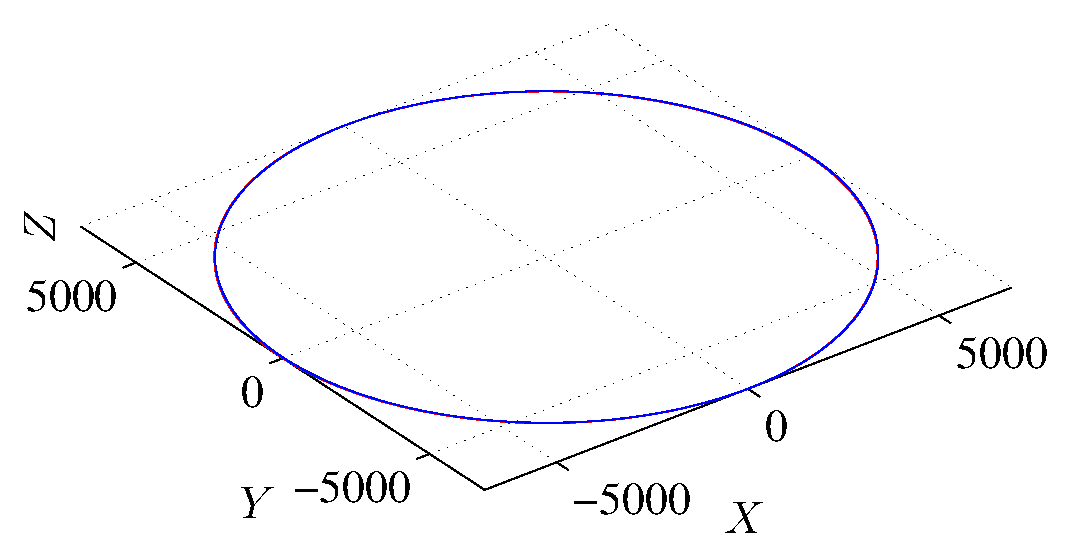
\includegraphics[width=0.3\textwidth]{OT_itraj_PE_r0_JAS_20}}
	\hspace*{0.15\textwidth}
		\subfigure[Orbital trajectory in the LVLH frame]{
		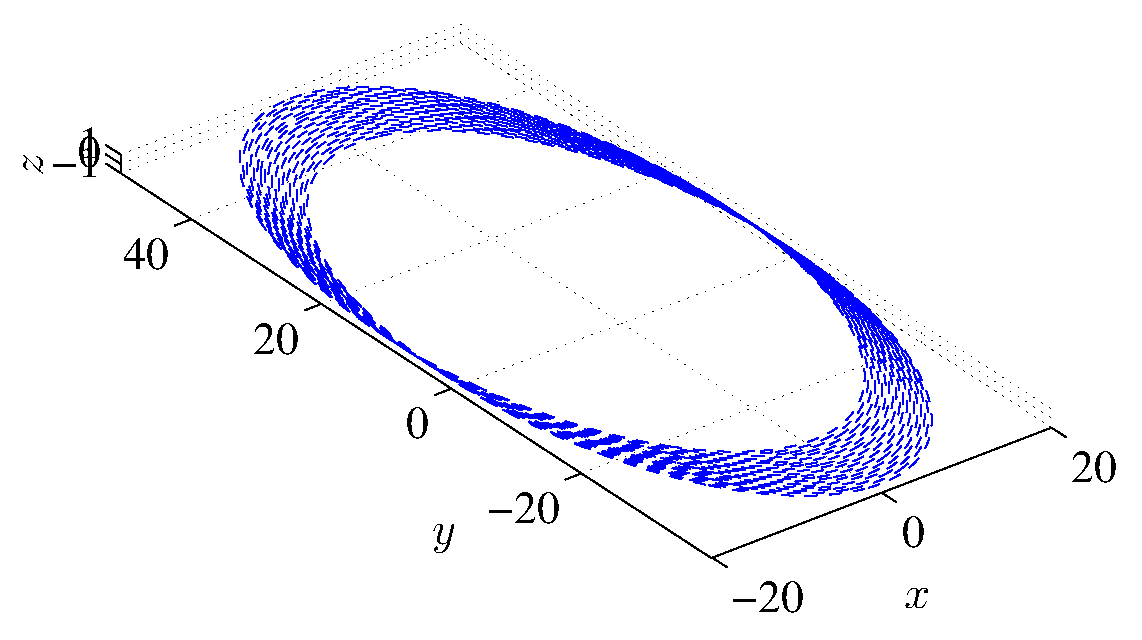
\includegraphics[width=0.25\textwidth]{OT_traj_PE_r0_JAS_20}}
}
\centerline{
	\subfigure[Estimation errors]{
		\includegraphics[width=0.3\textwidth]{EKF_PE_r0_20_e.pdf}}
	\hspace*{0.15\textwidth}
		\subfigure[Magnitude of state (red:true, blue:estimate)]{
		\includegraphics[width=0.3\textwidth]{EKF_PE_r0_20_xx_norm.pdf}}
}
\caption{Estimation results: $r_{x_0}=20\,\mathrm{km}$}\label{fig:r0_20}
\end{figure}
\begin{figure}
\centerline{
	\subfigure[Orbital trajectory in the inertial frame (red:chief, blue:deputy)]{
		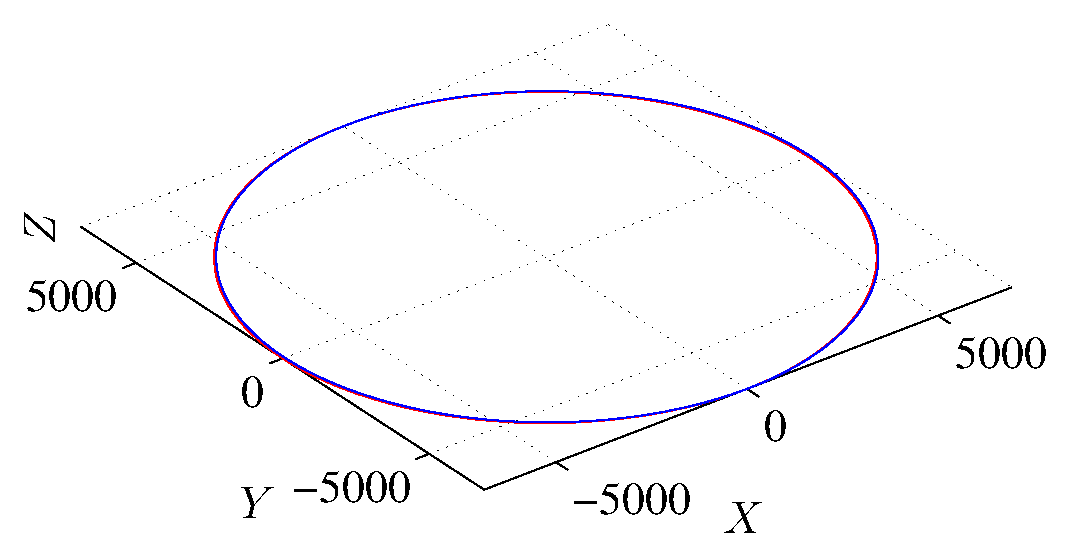
\includegraphics[width=0.3\textwidth]{OT_itraj_PE_r0_JAS_50}}
	\hspace*{0.15\textwidth}
		\subfigure[Orbital trajectory in the LVLH frame]{
		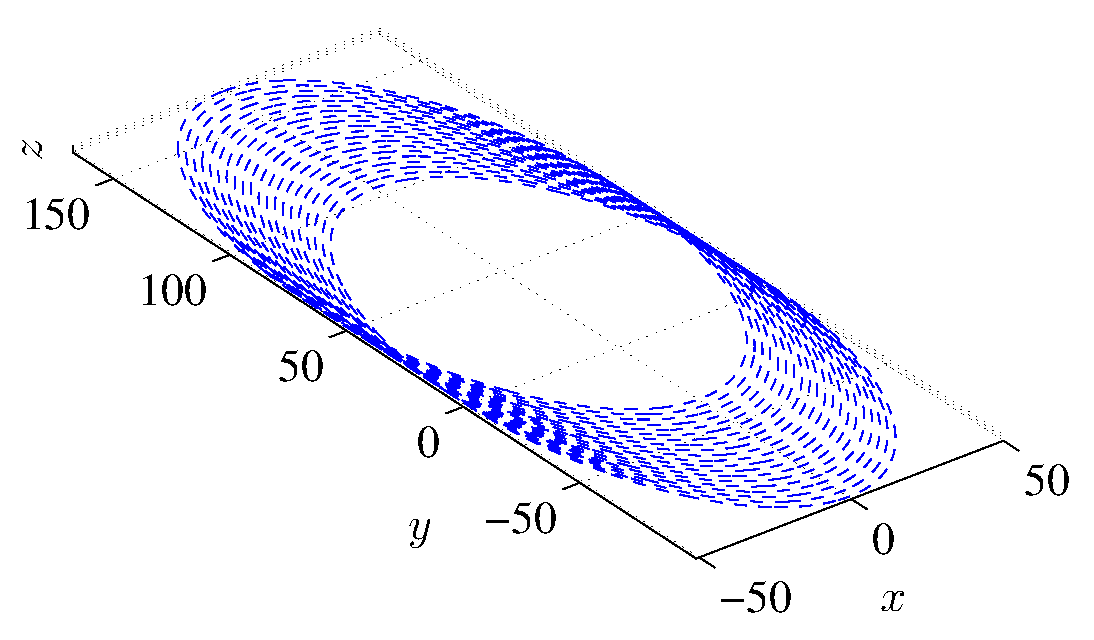
\includegraphics[width=0.25\textwidth]{OT_traj_PE_r0_JAS_50}}
}
\centerline{
	\subfigure[Estimation errors]{
		\includegraphics[width=0.3\textwidth]{EKF_PE_r0_50_e.pdf}}
	\hspace*{0.15\textwidth}
		\subfigure[Magnitude of state (red:true, blue:estimate)]{
		\includegraphics[width=0.3\textwidth]{EKF_PE_r0_50_xx_norm.pdf}}
}
\caption{Estimation results: $r_{x_0}=50\,\mathrm{km}$}\label{fig:r0_50}
\end{figure}
\begin{figure}
\centerline{
	\subfigure[Orbital trajectory in the inertial frame (red:chief, blue:deputy)]{
		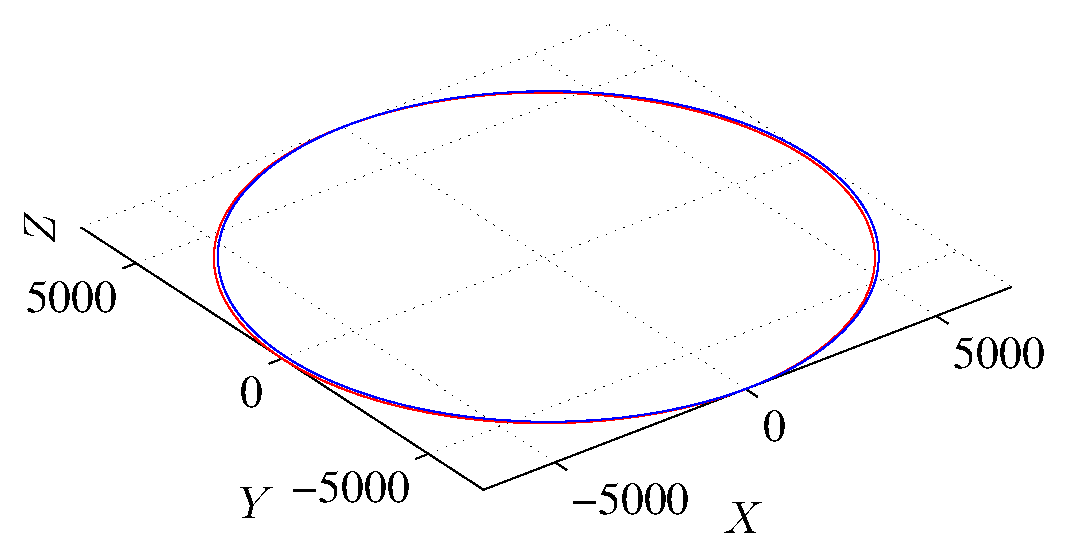
\includegraphics[width=0.3\textwidth]{OT_itraj_PE_r0_JAS_100}}
	\hspace*{0.15\textwidth}
		\subfigure[Orbital trajectory in the LVLH frame]{
		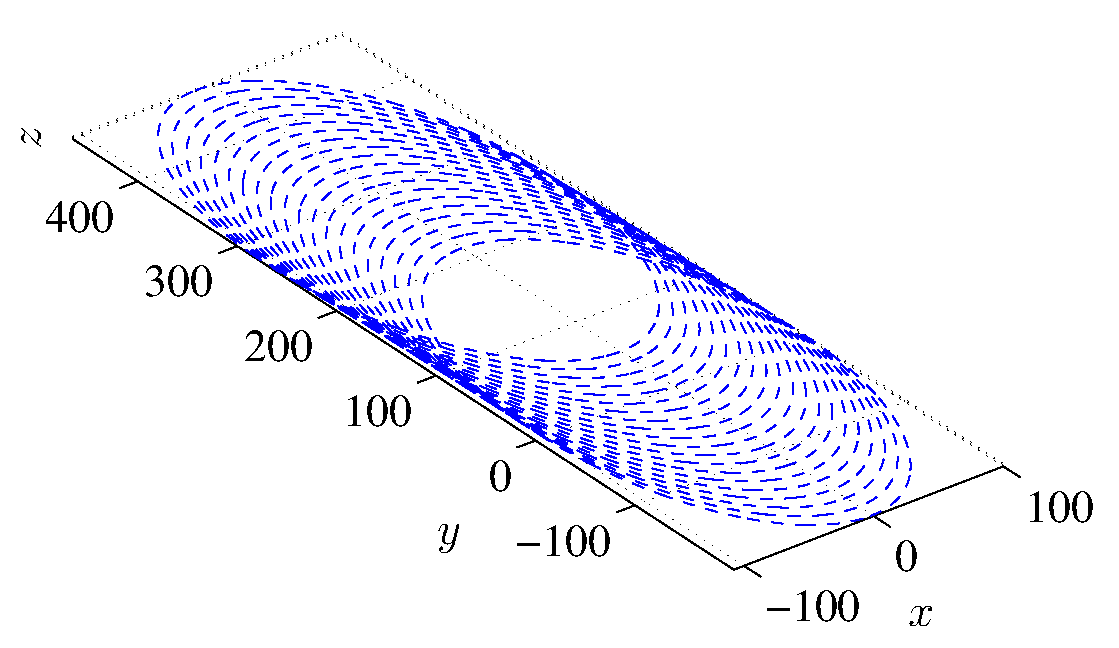
\includegraphics[width=0.25\textwidth]{OT_traj_PE_r0_JAS_100}}
}
\centerline{
	\subfigure[Estimation errors]{
		\includegraphics[width=0.3\textwidth]{EKF_PE_r0_100_e.pdf}}
	\hspace*{0.15\textwidth}
		\subfigure[Magnitude of state (red:true, blue:estimate)]{
		\includegraphics[width=0.3\textwidth]{EKF_PE_r0_100_xx_norm.pdf}}
}
\caption{Estimation results: $r_{x_0}=100\,\mathrm{km}$}\label{fig:r0_100}
\end{figure}

%\begin{figure}
%\centerline{
%	\subfigure[Estimation errors]{
%		\includegraphics[width=0.3\textwidth]{EKF_PE_r0_100_e_J2.pdf}}
%	\hspace*{0.15\textwidth}
%		\subfigure[Magnitude of state (red:true, blue:estimate)]{
%		\includegraphics[width=0.3\textwidth]{EKF_PE_r0_100_xx_norm_J2.pdf}}
%}
%\caption{Estimation results with $J_2$ perturbations: $r_{x_0}=100\,\mathrm{km}$}\label{fig:r0_100}
%\end{figure}
}


%\section{Numerical Results}
%
%We choose numerous cases of relative motion between chief and deputy satellite orbits.
%With each case, we evaluate the observability measure and process angles-only measurements with the EKF, using both the two-body equations of motion and higher fidelity propagation with $J_2$ effects as the truth models.
%%In particular, the $J_2$ gravitational harmonics will be included in the satellite propagation, so the EKF must handle simulated process uncertainty.
%To begin each simulation, an initial orbit determination (IOD) estimate is determined by various angles-only observations.
%These IOD estimates serve as initial estimates for the EKF.
%Then, we evaluate the performance of the EKF for these scenarios, specifically focusing on the observability measure and issues arising from initial conditions.
%
%Two IOD methods are developed in~\cite{NewLovPra14,PraLovNew14}, referred to as \emph{IOD1} and \emph{IOD2}, and employed to provide initial conditions for $13$ cases, outlined in Table \ref{tab:IODerr}.
%%Two IOD methods are referred to as \emph{IOD1} and \emph{IOD2}, and employed to provide initial conditions for $13$ cases, outlined in Table \ref{tab:IODerr}.
%These cases yield relative orbit trajectories illustrated in Figures \ref{fig:0CasesTraj}, \ref{fig:1CasesTraj}, \ref{fig:2CasesTraj}, \ref{fig:3CasesTraj}, and \ref{fig:4CasesTraj}.
%The most important distinction between the various cases is that in Case $\mathbf{1}$ the two-body solution and the linearized dynamics of the Hill-Clohessy-Wiltshire (HCW) solution are very close and the trajectory remains largely planar with a circular shape.
%
%\begin{figure}[h]
%\centerline{
%	\subfigure[Case 0A]{
%		\includegraphics[width=0.3\textwidth]{OM_IOD_0A_traj.pdf}}
%	\hfill
%	\subfigure[Case 0B]{
%		\includegraphics[width=0.3\textwidth]{OM_IOD_0B_traj.pdf}}
%	\hfill
%	\subfigure[Case 0C]{
%		\includegraphics[width=0.3\textwidth]{OM_IOD_0C_traj.pdf}}
%}
%\caption{The trajectories of the Cases 0A, 0B, and 0C (solid red: HCW, dashed blue: two-body solution) show that the linear and nonlinear solutions are close.
%The resulting trajectories are not cyclic as the trajectories change in the $y$-direction with time.}
%\label{fig:0CasesTraj}
%\end{figure}
%
%\begin{figure}[h]
%\label{fig:CaseTraj}
%\centerline{
%	\subfigure[Case 1]{
%		\includegraphics[width=0.3\textwidth]{OM_IOD_1_traj.pdf}}
%}
%\caption{The trajectory of the Case 1 (solid red: HCW, dashed blue: two-body solution) shows that the linear and nonlinear solutions are very close, where both solutions are largely planar and cyclic.}
%\label{fig:1CasesTraj}
%\end{figure}
%
%
%\begin{figure}[h]
%\centerline{
%	\subfigure[Case 2A]{
%		\includegraphics[width=0.3\textwidth]{OM_IOD_2A_traj.pdf}}
%	\hfill
%	\subfigure[Case 2B]{
%		\includegraphics[width=0.3\textwidth]{OM_IOD_2B_traj.pdf}}
%	\hfill
%	\subfigure[Case 2C]{
%		\includegraphics[width=0.3\textwidth]{OM_IOD_2C_traj.pdf}}
%}
%\caption{The trajectories of the Cases 2A, 2B, and 2C (solid red: HCW, dashed blue: two-body solution) show differences between the linear and nonlinear solutions that vary about the $y$-axis, increasing the observabilities.}
%\label{fig:2CasesTraj}
%\end{figure}
%
%\begin{figure}[h]
%\centerline{
%	\subfigure[Case 3A]{
%		\includegraphics[width=0.3\textwidth]{OM_IOD_3A_traj.pdf}}
%	\hfill
%	\subfigure[Case 3B]{
%		\includegraphics[width=0.3\textwidth]{OM_IOD_3B_traj.pdf}}
%	\hfill
%	\subfigure[Case 3C]{
%		\includegraphics[width=0.3\textwidth]{OM_IOD_3C_traj.pdf}}
%}
%\caption{The trajectories of the Cases 3A, 3B, and 3C (solid red: HCW, dashed blue: two-body solution) exhibit large observabilities due to nonlinear solutions that move far away from the linearized solutions.}
%\label{fig:3CasesTraj}
%\end{figure}
%
%\begin{figure}[h]
%\centerline{
%	\subfigure[Case 4A]{
%		\includegraphics[width=0.3\textwidth]{OM_IOD_4A_traj.pdf}}
%	\hfill
%	\subfigure[Case 4B]{
%		\includegraphics[width=0.3\textwidth]{OM_IOD_4B_traj.pdf}}
%	\hfill
%	\subfigure[Case 4C]{
%		\includegraphics[width=0.3\textwidth]{OM_IOD_4C_traj.pdf}}
%}
%\caption{The trajectories of the Cases 4A, 4B, and 4C (solid red: HCW, dashed blue: two-body solution) experience the largest observabilities due to nonlinear solutions that move farther away from the linearized solutions than any of the trajectories from other cases considered in this paper.}
%\label{fig:4CasesTraj}
%\end{figure}
%
%
%
%The initial error functions between the true orbit and and IOD predictions are defined as
%\begin{align}
%e_{mag,0}=\abs\left(1-{\frac{\norm{\r^+_0}}{\norm{\r_0}}}\right), \quad e_{dir,0}=\cos^{-1}\left(\frac{\r_0}{\norm{\r_0}}\cdot \frac{\r^+_0}{\norm{\r^+_0}}\right).
%\end{align}
%
%\begin{center}
%\begin{threeparttable}[h]
%\caption{Case Observabilities and Initial Errors}
%\begin{tabularx}{0.92\textwidth}
%{
%>{$}c<{$}
%*{1}{>{$}c<{$}} |
%*{2}{>{$}c<{$}} |
%*{2}{>{$}c<{$}}
%}
%\toprule
%\multirow{2}{*}{Case} & \multirow{2}{*}{$\mathrm{cond}\braces{\mathcal{W}}$} & \multicolumn{2}{c}{\multirow{1}{*}{IOD1}} & \multicolumn{2}{c}{\multirow{1}{*}{IOD2}} \\
%& &  e_{mag,0} & e_{dir,0} & e_{mag,0} & e_{dir,0} \\\midrule
%0A & 10^{11.1486} & 0.0003 & 1.4901\times10^{-8} & 0.0012  & 2.1073\times10^{-8} \\
%0B & 10^{10.9387} & 0.0233 & 0 & 0.0088 & 0 \\
%0C & 10^{10.9851} & 0.0152 & 2.1073\times10^{-8} & 0.0139 & 1.4901\times10^{-8}  \\
%\midrule
%\mathbf{1} & 10^{16.6871} & 0.0001 & 0 & 0 & 0  \\
%\midrule
%2A & 10^{10.6492} & 0.0550 & 1.8150\times10^{-4} & 0.0238 & 1.8150\times10^{-4}  \\
%2B & 10^{10.4163} & 0.9571 & 0.0734                     & 0.9571 & 0.0734  \\
%2C & 10^{10.2155} & 0.0219 & 0.0044 & 0.0065 & 0.0044 \\
%\midrule
%3A & 10^{8.3490} & 0.0191 & 0.0031 & 0.1830 & 0.0031  \\
%3B & 10^{8.5372} & 0.0612 & 0.0533 & 0.2315 & 0.0533  \\
%3C & 10^{8.6586} & 6.8962 & 0.7348 & 5.4921 & 0.7348  \\
%\midrule
%4A & 10^{7.9062} & 8.7347 & 0.4587 & 0.1575 & 0.4587  \\
%4B & 10^{7.9903} & 0.9276 & 0.1819 & 0.0621 & 0.1819  \\
%4C & 10^{8.0645} & 0.1161 & 0.0554 & 0.0354 & 0.0554  \\
%\bottomrule
%\end{tabularx}
%{\small
%\begin{tablenotes}
%    \item Note: $0$ indicates numbers small enough to be below Matlab numerical accuracy.
%  \end{tablenotes}}
%\label{tab:IODerr}
%\end{threeparttable}
%\end{center}
%
%
%The Kalman filter is used in each case. The initial state covariance matrix is chosen as
%\begin{align*}
%P_0^+=\diag[50^2,\ 50^2,\ 50^2,\ (50n)^2,\ (50n)^2,\ (50n)^2],
%\end{align*}
%and the process and measurement covariance matrices are chosen as
%\begin{align*}
%Q_k=\diag[10^{-7},\ 10^{-7},\ 10^{-7},\ 10^{-9},\ 10^{-9},\ 10^{-9}], \quad R_k=\tan^2{2^\circ}I_{3\times3}\ \forall\ k.
%\end{align*}
%%\begin{align*}
%%Q_k=10^q\diag[10^{-8},\ 10^{-8},\ 10^{-8},\ 10^{-10},\ 10^{-10},\ 10^{-10}], \quad R_k=\tan^2{2^\circ}I_{3\times3}\ \forall\ k
%%\end{align*}
%%where $q\in[-1,\ 0,\ 1,\ 2]$ is varied in the simulations, thereby changing the impact of measurement updates inside the Kalman filter.
%
%Each case is simulated for every IOD estimate. The running time is $59540$ seconds (slightly more than $\frac23$ of a day) with time steps of $10$ seconds between measurements. The following RMS errors are collected from each trial:
%\begin{align}
%\bar e_{mag}&=\left(\frac1N\sum_{k=1}^N\left\{1-{\frac{\norm{\r^+_k}}{\norm{\r_k}}}\right\}^2\right)^{\frac12},
%\\
%\bar e_{dir}&=\left(\frac1N\sum_{k=1}^N
%\left\{\cos^{-1}\left(\frac{\r_k}{\norm{\r_k}}\cdot \frac{\r^+_k}{\norm{\r^+_k}}\right)\right\}^{2}
%\right)^{\frac12},
%\end{align}
%for $N$ time steps.
%These metrics are tabulated in Tables \ref{tab:ResultsTBP} and \ref{tab:ResultsJ2}.
%Over the simulated time period, figures were generated for these analyses that  serve to compare the true and estimated state magnitudes and the maximum eigenvalues of the state covariance matrices as a measure of uncertainty for the state estimates.
%Because of paper constraints, a sample of these plots are shown that highlight various aspects of the observability and filter performance.
%
%
%
%%The figure below illustrates preliminary results for angles-only relative orbit estimation with $J_2$ perturbation in the measurements.
%%Note that the EKF performs well in this particular case, as evidenced by the close agreement between the true and estimated trajectory (Figure 1a) and the decrease in the maximum eigenvalue of the covariance matrix over time (Figure 1b).
%%For the various cases to be chosen, we will evaluate the performance of the EKF (using metrics such as those illustrated in Figure 1) and seek a consistent correlation between the filter performance and the new observability measure proposed above.
%
%
%
%%\begin{center}
%%\begin{threeparttable}[h]
%%\caption{Error variables for EKF with varying $Q_k$ Considering Only Two-Body Problem Forces}
%%\begin{tabularx}{\textwidth}
%%{
%%>{$}c<{$}
%%*{1}{>{$}c<{$}} |
%%*{4}{>{$}c<{$}} |
%%*{4}{>{$}c<{$}}
%%}
%%% & \bar e_{mag} & \bar e_{dir}
%%\toprule
%%\multirow{2}{*}{Case} & \multirow{2}{*}{IOD} & \multicolumn{4}{c}{$\bar e_{mag}$} & \multicolumn{4}{c}{$\bar e_{dir}$} \\
%%& & q=-1 & q=0 & q=1 & q=2 & q=-1 & q=0 & q=1 & q=2 \\\midrule
%%0A & IOD 1 & 0.0895 &  0.0611  &  0.3766  &  0.2861  &  0.0430  &  0.0135  &  0.0144  &  0.0183 \\
%%0A & IOD 2 & 0.1793 &  0.2811  &  0.5145  &  0.7716  &  0.0203  &  0.0313  &  0.0691  &  0.1046 \\
%%0B & IOD 1 & 0.3241 &  0.0531  &  0.5186  &  0.0620  &  0.1695  &  0.0143  &  0.0810  &  0.0172 \\
%%0B & IOD 2 & 0.2330 &  0.2115  &  0.3092  &  0.2733  &  0.1007  &  0.0879  &  0.0804  &  0.1048 \\
%%0C & IOD 1 & 0.0973 &   0.0748 &   0.2723 &   0.0607 &   0.0292 &   0.0068  &  0.1362 &   0.0443 \\
%%0C & IOD 2 & 0.1473 &   0.1017 &   0.1707 &   0.3545  &  0.0702  &  0.0517  &  0.0614  &  0.1224 \\
%%\midrule
%%\mathbf{1} & IOD 1 & \hilight{8.922} &   \hilight{2.964}   & \hilight{4.078}  &  \hilight{3.571} &   0.0071  &  0.0089  &  0.0109  &  0.0418 \\
%%\mathbf{1} & IOD 2 & \hilight{13.635} &  \hilight{14.121} &  \hilight{42.486} &  \hilight{42.573} &   0.0113 &   0.0107  &  0.0445  &  0.0115 \\
%%\midrule
%%2A & IOD 1 & 0.2045 &   0.0629 &   0.1592  &  0.1329  &  0.0041 &   0.0041  &  0.0043  &  0.0039 \\
%%2A & IOD 2 & 0.1013 &   0.1797  &  0.1348  &  0.2247  &  0.0050 &   0.0048 &   0.0065 &   0.0061 \\
%%2B & IOD 1 & \hilight{0.9886} &   \hilight{0.9895}   & \hilight{0.9843}  &  \hilight{0.9851}  &  0.0114 &   0.0116  &  0.0114  &  0.0116 \\
%%2B & IOD 2 & \hilight{0.9557} &   \hilight{0.9685} &   \hilight{0.9278}  &  \hilight{0.9431} &   0.0105  &  0.0108 &   0.0113 &   0.0153 \\
%%2C & IOD 1 & 0.0219 &   0.0184  &  0.0258  &  0.0238 &   0.0026 &   0.0031  &  0.0044 &   0.0038 \\
%%2C & IOD 2 & 0.0303 &   0.0287  &  0.0360  &  0.0470  &  0.0044  &  0.0054  &  0.0059 &   0.0062 \\
%%\midrule
%%3A & IOD 1 &  0.2377 &   0.1684  &  0.0486 &   0.0695 &   0.0094 &   0.0070 &   0.0040 &  0.0039 \\
%%3A & IOD 2 &  0.0854  &  0.0874 &   0.0603  &  0.0544  &  0.0035 &   0.0033  &  0.0053  &  0.0042 \\
%%3B & IOD 1 &  0.0724 &   0.0260 &   0.0680  &  0.0289  &  0.0035 &   0.0029  &  0.0033  &  0.0027 \\
%%3B & IOD 2 &  0.0385  &  0.0432  &  0.1459  &  0.0284  &  0.0038  &  0.0037  &  0.0070  &  0.0047 \\
%%3C & IOD 1 &  \hilight{2.2433}  &  \hilight{1.5231} &   \hilight{2.0611} &   \hilight{1.5110}  &  0.1803  &  0.1172  &  0.1595  &  0.1103 \\
%%3C & IOD 2 &  \hilight{4.0635} &   \hilight{1.7717}  & \hilight{10.567}  &  \hilight{4.0277} &   0.4475 &   0.1506 &   0.9011 &   0.4028 \\
%%\midrule
%%4A & IOD 1 &  \hilight{6.0259} &   \hilight{0.0464}  &  \hilight{6.0706}  &  \hilight{0.0325}  &  1.3353  &  0.0087   & 1.3182  &  0.0065 \\
%%4A & IOD 2 &  6.3646 &   0.0173  & 11.8882 &   0.0256 &   1.3423  &  0.0064  &  1.5319 &   0.0066 \\
%%4B & IOD 1 &  \hilight{0.2922}  &  \hilight{0.0258}  &  \hilight{0.2723}  &  \hilight{0.0182}   & 0.0929 &   0.0032  &  0.0789  &  0.0036 \\
%%4B & IOD 2 &  0.1815  &  0.0217  &  0.3155 &   0.0771  &  0.0268   & 0.0034  &  0.1061 &   0.0044 \\
%%4C & IOD 1 &  0.0247  &  \hilight{0.0421}  &  2.3699  &  0.0182  &  0.0032  &  0.0032  &  0.8486 &   0.0028 \\
%%4C & IOD 2 &  0.0200 &   0.0128  &  0.0278  &  0.0299 &   0.0040  &  0.0029  &  0.0034  &  0.0033 \\
%%\bottomrule
%%\end{tabularx}
%%{\small
%%\begin{tablenotes}
%%    \item \hilight{Filter diverges}
%%  \end{tablenotes}}
%%\label{tab:ResultsTBP}
%%\end{threeparttable}
%%\end{center}
%%
%%\begin{center}
%%\begin{threeparttable}[h]
%%\caption{Error variables for EKF with varying $Q_k$ with $J_2$ Perturbations Included}
%%\begin{tabularx}{\textwidth}
%%{
%%>{$}c<{$}
%%*{1}{>{$}c<{$}} |
%%*{4}{>{$}c<{$}} |
%%*{4}{>{$}c<{$}}
%%}
%%\toprule
%%\multirow{2}{*}{Case} & \multirow{2}{*}{IOD} & \multicolumn{4}{c}{$\bar e_{mag}$} & \multicolumn{4}{c}{$\bar e_{dir}$} \\
%%& & q=-1 & q=0 & q=1 & q=2 & q=-1 & q=0 & q=1 & q=2 \\\midrule
%%0A & IOD 1 & 0.0553  &  0.1105  &  0.1918  &  0.2298  &  0.0059  &  0.0062  &  0.0069  &  0.0069 \\
%%0A & IOD 2 & 0.2177  &  0.3227  &  0.3140  &  0.5013  &  0.0082  &  0.0074  &  0.0129  &  0.0085 \\
%%0B & IOD 1 & 0.0473  &  0.1246  &  0.7262  &  0.0655  &  0.0077  &  0.0088  &  0.0505  &  0.0066\\
%%0B & IOD 2 & 0.8872  &  0.4186  &  0.1571  &  0.1561  &  0.0390  &  0.0168  &  0.0086  &  0.0293 \\
%%0C & IOD 1 & 0.0652  &  0.0809  &  0.0900  &  0.1113  &  0.0082  &  0.0079  &  0.0061  &  0.0106 \\
%%0C & IOD 2 & 0.0367  &  0.0204  &  0.1002  &  0.7253  &  0.0145  &  0.0084  &  0.0154  &  0.0579 \\
%%\midrule
%%\mathbf{1} & IOD 1 & \hilight{9.1098}  &  \hilight{2.900}  &  \hilight{4.059}  &  \hilight{3.567}  &  0.0071  &  0.0090  &  0.0109  &   0.0418 \\
%%\mathbf{1} & IOD 2 & \hilight{13.594} & \hilight{14.033} & \hilight{42.381} & \hilight{42.979}  & 0.0113   & 0.0107   & 0.0445   &   0.0115 \\
%%\midrule
%%2A & IOD 1 & 0.2301  &  0.0423  &  0.1978  &  0.1740  &  0.0048  &  0.0049  &  0.0047  &  0.0042 \\
%%2A & IOD 2 & 0.1058  &  0.2164  &  0.1638  &  0.2644  &  0.0051  &  0.0049  &  0.0065  &  0.0061 \\
%%2B & IOD 1 & \hilight{0.9895}  &  \hilight{0.9902}  &  \hilight{0.9853}  &  \hilight{0.9859}  &  0.0115  &  0.0117  &  0.0115  &  0.0117 \\
%%2B & IOD 2 & \hilight{0.9585}  &  \hilight{0.9701}  &  \hilight{0.9307}  &  \hilight{0.9455}  &  0.0106  &  0.0109  &  0.0114  &  0.0153 \\
%%2C & IOD 1 & 0.0481  &  0.0474  &  0.0563  &  0.0415  &  0.0041  &  0.0042  &  0.0047  &  0.0042 \\
%%2C & IOD 2 & 0.0535  &  0.0397  &  0.0536  &  0.0705  &  0.0044  &  0.0056  &  0.0059  &  0.0062 \\
%%\midrule
%%3A & IOD 1 &  0.2462  &  0.1827  &  0.0516  &  0.0699 &   0.0097 &   0.0077  &  0.0041 &   0.0041 \\
%%3A & IOD 2 &  0.1038  &  0.0986  &  0.0643  &  0.0692 &   0.0036  &  0.0034  &  0.0053  &  0.0041 \\
%%3B & IOD 1 &  0.0770  &  0.0310  &  0.0739  &  0.0458 &   0.0038 &   0.0034  &  0.0035  &  0.0031 \\
%%3B & IOD 2 &  0.0461  &  0.0585   & 0.1485 &   0.0391  &  0.0039  &  0.0040  &  0.0071  &  0.0047 \\
%%3C & IOD 1 &  \hilight{2.239}  &  \hilight{1.522}  &  \hilight{2.063}  &  \hilight{1.514}  &  0.1817  &  0.1179  &  0.1614  &  0.1116 \\
%%3C & IOD 2 &  \hilight{4.188}  &  \hilight{1.821}  & \hilight{10.136}  &  \hilight{4.510} &   0.4873 &   0.1592  &  0.9195 &   0.5532 \\
%%\midrule
%%4A & IOD 1 &  \hilight{6.013}  &  \hilight{0.0454}  &  \hilight{6.359}  &  \hilight{0.031}  &  1.3131  &  0.0086  &  1.4235 &   0.0066 \\
%%4A & IOD 2 &  6.3272  &  0.0197  & 12.0062 &  0.0248  &  1.3116  &  0.0065  &  1.5310  &  0.0066 \\
%%4B & IOD 1 &  \hilight{0.2936}  &  \hilight{0.0272}  &  \hilight{0.2773}  &  \hilight{0.0217}  &  0.0935  &  0.0032  &  0.0814  &  0.0038 \\
%%4B & IOD 2 &  0.1853  &  0.0210  &  0.5244  &  0.0785  &  0.0293  &  0.0036  &  0.2305  &  0.0045 \\
%%4C & IOD 1 &  0.0260  &  \hilight{0.0410}  &  2.0105  &  0.0164  &  0.0034  &  0.0031  &  0.9144  &  0.0030 \\
%%4C & IOD 2 &  0.0210  &  0.0145  &  0.0303  &  0.0349  &  0.0042  &  0.0030  &  0.0036  &  0.0034 \\
%%\bottomrule
%%\end{tabularx}
%%{\small
%%\begin{tablenotes}
%%    \item \hilight{Filter diverges}
%%  \end{tablenotes}}
%%\label{tab:ResultsJ2}
%%\end{threeparttable}
%%\end{center}
%
%\begin{center}
%\begin{threeparttable}[h]
%\caption{Error variables for EKF Considering Only Two-Body Problem Forces}
%\begin{tabularx}{.74\textwidth}
%{
%>{$}c<{$}
%*{1}{>{$}c<{$}} |
%*{2}{>{$}c<{$}} |
%*{2}{>{$}c<{$}}
%}
%\toprule
%\multirow{2}{*}{Case} & \multirow{2}{*}{$\mathrm{cond}\braces{\mathcal{W}}$} & \multicolumn{2}{c}{IOD1} & \multicolumn{2}{c}{IOD2} \\
%& & \bar e_{mag} & \bar e_{dir} & \bar e_{mag} & \bar e_{dir} \\\midrule
%0A & 10^{11.1486} &  0.3766  &  0.0144  &  0.5145  &  0.0691 \\
%0B & 10^{10.9387} &  0.5186  &  0.0810  &  0.3092  &  0.0804\\
%0C & 10^{10.9851} &  0.2723  &  0.1362 &  0.1707 &  0.0614\\
%\midrule
%\mathbf{1} & 10^{16.6871} & \cellcolor{green} 4.078  & \cellcolor{green}  0.0109 & \cellcolor{green} 42.486 & \cellcolor{green}  0.0445 \\
%\midrule
%2A & 10^{10.6492} &  0.1592  &   0.0043  &  0.1348  &   0.0065   \\
%2B & 10^{10.4163} & \cellcolor{green} 0.9843   & \cellcolor{green}  0.0114  & \cellcolor{green}  0.9278 & \cellcolor{green}   0.0113 \\
%2C & 10^{10.2155} & 0.0258 &  0.0044 & 0.0360 &  0.0059 \\
%\midrule
%3A & 10^{8.3490} &  0.0486 & 0.0040   &  0.0603  &  0.0053 \\
%3B & 10^{8.5372} &  0.0680  &  0.0033 &  0.1459 &  0.0070 \\
%3C & 10^{8.6586} & \cellcolor{green}  2.0611 & \cellcolor{green}  0.1595   & \cellcolor{green}  10.567  & \cellcolor{green}   0.9011 \\
%\midrule
%4A & 10^{7.9062} & \cellcolor{green}  6.0706  & \cellcolor{green} 1.3182  &  11.8882   &  1.5319  \\
%4B & 10^{7.9903} & \cellcolor{green}  0.2723  & \cellcolor{green}  0.0789   &  0.3155  &  0.1061 \\
%4C & 10^{8.0645} &  2.3699 &  0.8486   &  0.0278 &  0.0034 \\
%\bottomrule
%\end{tabularx}
%{\small
%\begin{tablenotes}
%    \item \hilight{Filter diverges}
%  \end{tablenotes}}
%\label{tab:ResultsTBP}
%\end{threeparttable}
%\end{center}
%
%\begin{center}
%\begin{threeparttable}[h]
%\caption{Error variables for EKF Considering $J_2$ Perturbations}
%\begin{tabularx}{.74\textwidth}
%{
%>{$}c<{$}
%*{1}{>{$}c<{$}} |
%*{2}{>{$}c<{$}} |
%*{2}{>{$}c<{$}}
%}
%\toprule
%\multirow{2}{*}{Case} & \multirow{2}{*}{$\mathrm{cond}\braces{\mathcal{W}}$} & \multicolumn{2}{c}{IOD1} & \multicolumn{2}{c}{IOD2} \\
%& & \bar e_{mag} & \bar e_{dir} & \bar e_{mag} & \bar e_{dir} \\\midrule
%0A & 10^{11.1486} &  0.1918  &  0.0069  &  0.3140  &  0.0129 \\
%0B & 10^{10.9387} &  0.7262  &  0.0505  &  0.1571  &  0.0086\\
%0C & 10^{10.9851} &  0.0900  &  0.0061 &  0.1002  &  0.0154\\
%\midrule
%\mathbf{1} & 10^{16.6871} & \cellcolor{green} 4.059  & \cellcolor{green}  0.0109 & \cellcolor{green} 42.381 & \cellcolor{green}  0.0445 \\
%\midrule
%2A & 10^{10.6492} &  0.1978  &  0.0047  &  0.1638  &   0.0065   \\
%2B & 10^{10.4163} & \cellcolor{green}  0.9853  & \cellcolor{green}  0.9307 & \cellcolor{green}  0.9278 & \cellcolor{green}   0.0114 \\
%2C & 10^{10.2155} & 0.0563 &  0.0047 & 0.0536 &  0.0059 \\
%\midrule
%3A & 10^{8.3490} &  0.0516 & 0.0041   &  0.0643  &  0.0053 \\
%3B & 10^{8.5372} &  0.0739  &  0.0035 &  0.1485 &  0.0071 \\
%3C & 10^{8.6586} & \cellcolor{green}  2.063 & \cellcolor{green} 0.1614    & \cellcolor{green}  10.136  & \cellcolor{green}   0.9195 \\
%\midrule
%4A & 10^{7.9062} & \cellcolor{green}  6.359  & \cellcolor{green} 1.4235  &  12.0062   &  1.5310  \\
%4B & 10^{7.9903} & \cellcolor{green}  0.2773  & \cellcolor{green}  0.0814   &  0.5244  &  0.2305 \\
%4C & 10^{8.0645} &  2.0105 &  0.9144   &  0.0303 &  0.0036 \\
%\bottomrule
%\end{tabularx}
%{\small
%\begin{tablenotes}
%    \item \hilight{Filter diverges}
%  \end{tablenotes}}
%\label{tab:ResultsJ2}
%\end{threeparttable}
%\end{center}
%
%These data from the simulations show several important aspects and challenges with relative orbit determination involving angles-only measurements.
%First, an important observation from the data is that the IOD guess is critical to the success of the Kalman filter.
%Cases 2B, 3C, 4A, and 4B experience filter divergence when the IOD estimate is largely inaccurate, shown in Tables \ref{tab:IODerr}, \ref{tab:ResultsTBP}, and \ref{tab:ResultsJ2}, even when cases with similar observabilities do not experience filter divergence.
%The Kalman filter, which is based on linear dynamic systems, is modeled as a Markov chain and hence is memoryless.
%Therefore when nothing more than an inaccurate IOD prediction is poorly assumed to contain accurate information about the system, the recursive formulation of the Kalman filter is unable to converge.
%In these diverging cases, a greater level of observability or an algorithm that relies on a larger history of measurements may improve convergence.
%
%
%In contrast, every variation of Case $\mathbf{1}$ has a closer IOD than the IODs of other cases, but experiences the most severe divergence.
%Case $\mathbf{1}$ has a greater condition number of $\mathcal W$, which corresponds with low observability according to the proposed observability measure.
%A series of angles-only measurements may correspond with a large range of possible relative orbits, even with a low variation in those measurements.
%Therefore, small levels of noise in the sensor or uncertainties in the orbit prevent the Kalman filter from converging to an accurate estimate, even with an accurate IOD.
%The state magnitudes of both variations of Case $\mathbf{1}$ are illustrated against various converging cases in Figure \ref{fig:ExampesEachCase} to show how important this observability is to the filter performance.
%
%\begin{figure}[h]
%\centerline{
%	\subfigure[Case 0C, IOD1]{
%		\includegraphics[width=0.35\textwidth]{Case0Cq1IOD1TBPnormX.pdf}}
%	\hfill
%	\subfigure[Case 0C, IOD2]{
%	\includegraphics[width=0.35\textwidth]{Case0Cq1IOD2TBPnormX.pdf}}
%}
%\centerline{
%	\subfigure[Case $\mathbf{1}$, IOD1]{
%		\includegraphics[width=0.35\textwidth]{Case1q1IOD1TBPnormX.pdf}}
%	\hfill
%	\subfigure[Case $\mathbf{1}$, IOD2]{
%	\includegraphics[width=0.35\textwidth]{Case1q1IOD2TBPnormX.pdf}}
%}
%\centerline{
%	\subfigure[Case 2A, IOD1]{
%		\includegraphics[width=0.35\textwidth]{Case2Aq1IOD1TBPnormX.pdf}}
%	\hfill
%	\subfigure[Case 2A, IOD2]{
%	\includegraphics[width=0.35\textwidth]{Case2Aq1IOD2TBPnormX.pdf}}
%}
%\centerline{
%	\subfigure[Case 3A, IOD1]{
%		\includegraphics[width=0.35\textwidth]{Case3Aq1IOD1TBPnormX.pdf}}
%	\hfill
%	\subfigure[Case 3A, IOD2]{
%	\includegraphics[width=0.35\textwidth]{Case3Aq1IOD2TBPnormX.pdf}}
%}
%\centerline{
%	\subfigure[Case 4C, IOD1]{
%		\includegraphics[width=0.35\textwidth]{Case4Cq1IOD1TBPnormX.pdf}}
%	\hfill
%	\subfigure[Case 4C, IOD2]{
%	\includegraphics[width=0.35\textwidth]{Case4Cq1IOD2TBPnormX.pdf}}
%}
%\caption{The magnitudes of the relative states (solid red: true, blue dashed: estimated) are shown for various two-body propagated cases with close IOD estimates where the filter only diverges when the observability is low.}\label{fig:ExampesEachCase}
%\end{figure}
%
%
%Another observation from the data is that the $J_2$ perturbation, which is well-known to have a noticeable impact perturbing orbits from the two-body model for satellites around the earth, yields an insignificant change when compared to the data when only two-body forces are considered in the process model.
%In fact, every case when the filter diverged occurred with both the two-body problem and $J_2$ simulations.
%Examples of these results are tabulated in Tables \ref{tab:ResultsTBP} and \ref{tab:ResultsJ2} and illustrated in Figure \ref{fig:TBPvsJ2}.
%
%
%
%\begin{figure}[h]
%\centerline{
%	\subfigure[State magnitude with the two-body solution]{
%		\includegraphics[width=0.48\textwidth]{Case3Bq1IOD1TBPnormX.pdf}}
%	\hfill
%	\subfigure[State magnitude with the $J_2$ solution]{
%		\includegraphics[width=0.48\textwidth]{Case3Bq1IOD1HighFidelitynormX.pdf}}
%}
%\centerline{
%	\subfigure[Uncertainty measure with the two-body solution]{
%		\includegraphics[width=0.48\textwidth]{Case3Bq1IOD1TBPeigP.pdf}}
%	\hfill
%	\subfigure[Uncertainty measure with the $J_2$ solution]{
%		\includegraphics[width=0.48\textwidth]{Case3Bq1IOD1eigP.pdf}}
%}
%\caption{The magnitudes and maximum eigenvalues of the state covariance matrices of the relative states (solid red: true, blue dashed: estimated) in Case 3B with IOD1 serve as an example where the $J_2$ propagated simulations give very close results to those of the two-body solution.
%}\label{fig:TBPvsJ2}
%\end{figure}






\section{Conclusions}

It is well known that linearized relative orbital dynamics are not observable with angles-only
measurements. This paper studies the observability for nonlinear relative orbital dynamics, and it derives a set of sufficiency conditions to show that the relative orbit is indeed observable under certain geometric conditions. Also, a quantitative observability measure that represents the degree of observability is proposed. It is illustrated by several numerical examples. Future works include constructing observability criteria based on higher-order Lie derivatives of the measurement, and developing nonlinear filtering techniques that can capture the weak coupling between the dynamics of relative motion and the line-of-sight measurements effectively, as well as studying the effects of higher-order gravitational perturbations on the observability. 

%formulates a measure of nonlinear observability, and investigates a less conservative observability criteria by using higher-order Lie derivatives. Numerous relative orbit determination cases are illustrated numerically by an extended Kalman filter, which shows that the degree of observability by the proposed measure and an accurate IOD prediction are useful for predicting filter convergence.























%\section{Section title}
%\label{sec:1}
%Text with citations \cite{RefB} and \cite{RefJ}.
%\subsection{Subsection title}
%\label{sec:2}
%as required. Don't forget to give each section
%and subsection a unique label (see Sect.~\ref{sec:1}).
%\paragraph{Paragraph headings} Use paragraph headings as needed.
%\begin{equation}
%a^2+b^2=c^2
%\end{equation}

% For one-column wide figures use
%\begin{figure}
%% Use the relevant command to insert your figure file.
%% For example, with the graphicx package use
%  \includegraphics{example.eps}
%% figure caption is below the figure
%\caption{Please write your figure caption here}
%\label{fig:1}       % Give a unique label
%\end{figure}
%
% For two-column wide figures use
%\begin{figure*}
%% Use the relevant command to insert your figure file.
%% For example, with the graphicx package use
%  \includegraphics[width=0.75\textwidth]{example.eps}
%% figure caption is below the figure
%\caption{Please write your figure caption here}
%\label{fig:2}       % Give a unique label
%\end{figure*}
%
%% For tables use
%\begin{table}
%% table caption is above the table
%\caption{Please write your table caption here}
%\label{tab:1}       % Give a unique label
%% For LaTeX tables use
%\begin{tabular}{lll}
%\hline\noalign{\smallskip}
%first & second & third  \\
%\noalign{\smallskip}\hline\noalign{\smallskip}
%number & number & number \\
%number & number & number \\
%\noalign{\smallskip}\hline
%\end{tabular}
%\end{table}


%\begin{acknowledgements}
%If you'd like to thank anyone, place your comments here
%and remove the percent signs.
%\end{acknowledgements}

% BibTeX users please use one of
%\bibliographystyle{spbasic}      % basic style, author-year citations
%\bibliographystyle{spmpsci}      % mathematics and physical sciences
%\bibliographystyle{spphys}       % APS-like style for physics
\bibliography{BibSources}   % name your BibTeX data base



%% Non-BibTeX users please use
%\begin{thebibliography}{}
%%
%% and use \bibitem to create references. Consult the Instructions
%% for authors for reference list style.
%%
%\bibitem{RefJ}
%% Format for Journal Reference
%Author, Article title, Journal, Volume, page numbers (year)
%% Format for books
%\bibitem{RefB}
%Author, Book title, page numbers. Publisher, place (year)
%% etc
%\end{thebibliography}

\end{document}
% end of file template.tex

